\documentclass[10pt,a4paper]{article}
\usepackage[letterpaper, total={6in, 9in}]{geometry}
\usepackage{hyperref}
\usepackage{float}
\usepackage{mathdots}
%\usepackage{mathptmx}       % selects Times Roman as basic font
\usepackage{helvet}         % selects Helvetica as sans-serif font
\usepackage{courier}        % selects Courier as typewriter font
%\usepackage{type1cm}        % activate if the above 3 fonts are not available on your system
%\usepackage{makeidx}         % allows index generation
\usepackage{braket}
%\usepackage{citeref}
\usepackage{amscd,amssymb,amsmath,latexsym,bm}
\usepackage{mathtools} 
\usepackage[mathcal,mathscr]{euscript}
\usepackage{lipsum}
\usepackage{adjustbox}
\usepackage{amsfonts}
\usepackage{graphicx}
\usepackage{enumitem}
\usepackage{hyperref}
\usepackage[table,dvipsnames]{xcolor}
\usepackage{upgreek}
\usepackage{ulem}
\usepackage[utf8]{inputenc}
%\usepackage{movie15}
%\usepackage{subcaption}
\usepackage{tikz}
\usetikzlibrary{braids,backgrounds,arrows,fit}
\usepackage{xcolor-material}

\newcommand{\DD}[2]{\boxed{D_{#1}^{#2}}}
\renewcommand{\ket}[1]{\left\vert{#1}\right\rangle}
\renewcommand{\bra}[1]{\left\langle{#1}\right\vert}
\renewcommand{\braket}[2]{\left\langle{#1}\vert{#2}\right\rangle}
\newcommand{\avg}[1]{\left\langle{#1}\right\rangle}
\newcommand{\mat}{\overleftrightarrow}
%\newcommand{\Set}[1]{\left\lbrace{#1}\right\rbrace}
\newcommand{\abs}[1]{\left\vert{#1}\right\vert}
\newcommand{\id}{I}

\newcommand{\atPlanar}[2]{%arrow triple single strand diagram
	\begin{tikzpicture}[->,>=stealth']
	\draw[color=red] (0,0) rectangle (1.2,0.7);
	\filldraw (0.3,0) circle [radius=1pt];
	\filldraw (0.6,0) circle [radius=1pt];
	\filldraw (0.9,0) circle [radius=1pt];
	\filldraw (0.3,0.7) circle [radius=1pt];
	\filldraw (0.6,0.7) circle [radius=1pt];
	\filldraw (0.9,0.7) circle [radius=1pt];
	\draw (0.3*#1,0) .. controls +(0,0.2) and +(0,-0.2) .. (0.3*#2,0.7);
	\end{tikzpicture}
	}

\newcommand{\tPlanar}[3]{
	\draw[color=red] (0,{0.7*(#3-1)}) rectangle (1.2,0.7*#3);
	\filldraw (0.3,{0.7*(#3-1)}) circle [radius=1pt];
	\filldraw (0.6,{0.7*(#3-1)}) circle [radius=1pt];
	\filldraw (0.9,{0.7*(#3-1)}) circle [radius=1pt];
	\filldraw (0.3,0.7*#3) circle [radius=1pt];
	\filldraw (0.6,0.7*#3) circle [radius=1pt];
	\filldraw (0.9,0.7*#3) circle [radius=1pt];
	\draw (0.3*#1,{0.7*(#3-1)}) .. controls +(0,0.2) and +(0,-0.2) .. (0.3*#2,0.7*#3);
	}

\newcommand{\bPlanar}[3]{
	\draw[color=red] (0,{0.7*(#3-1)}) rectangle (0.9,0.7*#3);
	\filldraw (0.3,{0.7*(#3-1)}) circle [radius=1pt];
	\filldraw (0.6,{0.7*(#3-1)}) circle [radius=1pt];
	\filldraw (0.3,0.7*#3) circle [radius=1pt];
	\filldraw (0.6,0.7*#3) circle [radius=1pt];
	\draw (0.3*#1,{0.7*(#3-1)}) .. controls +(0,0.2) and +(0,-0.2) .. (0.3*#2,0.7*#3);
	}

\newcommand{\Drawbox}[2][1]{
	% optional: level, mandatory: N dots,
	% usage: \Drawbox[levels]{Ndots} , or \DrawBox{Ndots} with one level
	\foreach \level in {1,...,#1}{
		\draw[color=red] (0,0.7*\level-0.7) rectangle (#2*0.3+0.3,0.7*\level);
		\foreach \dot in {1,...,#2}{
			\filldraw (0.3*\dot,0.7*\level-0.7) circle [radius=1pt];
			\filldraw (0.3*\dot,0.7*\level) circle [radius=1pt];
		};
	};
}

\newcommand{\Drawline}[3][1]{
	% optional: level, mandatory: start end,
	% usage: \Drawline[level]{start}{end} , or \Drawline{start}{end} with one level
	\draw (0.3*#2,0.7*#1-0.7) .. controls +(0,0.2) and +(0,-0.2) .. (0.3*#3,0.7*#1);
}


\tikzset{%
	apple/.pic={
		\fill [MaterialBrown] (-1/8,0) 
		arc (180:120:1 and 3/2) coordinate [pos=3/5] (@)-- ++(1/6,-1/7) 
		arc (120:180:5/4 and 3/2) -- cycle;
		\fill [MaterialLightGreen500] (0,-9/10) 
		.. controls ++(180:1/8) and ++(  0:1/4) .. (-1/3,  -1)
		.. controls ++(180:1/3) and ++(270:1/2) .. (  -1,   0)
		.. controls ++( 90:1/3) and ++(180:1/3) .. (-1/2, 3/4)
		.. controls ++(  0:1/8) and ++(135:1/8) .. (   0, 4/7)
		.. controls ++( 45:1/8) and ++(180:1/8) .. ( 1/2, 3/4)
		.. controls ++(  0:1/3) and ++( 90:1/3) .. (   1,   0)
		.. controls ++(270:1/2) and ++(  0:1/3) .. ( 1/3,  -1)
		.. controls ++(180:1/4) and ++(  0:1/8) .. cycle;
		\fill [MaterialLightGreen600] (0, 4/7)
		.. controls ++( 45:1/8) and ++(180:1/8) .. ( 1/2, 3/4)
		.. controls ++(  0:1/3) and ++( 90:1/3) .. (   1,   0)
		.. controls ++(270:1/2) and ++(  0:1/3) .. ( 1/3,  -1)
		.. controls ++(180:1/4) and ++(  0:1/8) .. (   0,-9/10);
		\fill [MaterialGreen500, shift={(@)}, rotate=-30] 
		(0,0) arc (45:135:3/4 and 3/5) arc (225:315:3/4 and 3/5);
		\fill [MaterialGreen700, shift={(@)}, rotate=-30] 
		(0,0) arc (315:225:3/4 and 3/5) -- cycle;
	},
	orange/.pic={
		\fill [MaterialOrange500] (0,0) circle [radius=1];
		\fill [MaterialOrange600] (0,0) -- (45:1) arc (45:-135:1) -- cycle;
		\fill [MaterialOrange700, shift={(0,3/4)}] coordinate (@)
		ellipse [x radius=1/4, y radius=1/8];
		\begin{scope}
			\clip (0,0) circle [radius=1];
			\fill [MaterialOrange700, shift=(@)] (90:1/4 and 1/8) 
			\foreach \i [evaluate={\j=mod(\i,2)+1/4;}]in {0,...,12}{
				-- (90+\i*30:\j*3/4 and \j*3/8) } -- cycle;
		\end{scope}
		\fill [MaterialBrown] (-1/16, 3/4) -- ++(0,1/4) arc (180:0:1/16 and 1/32)
		-- ++(0,-1/4) arc (360:180:1/16 and 1/32) -- cycle;
		\fill [MaterialGreen500, shift=(@), rotate=-150] 
		(0,0) arc (45:135:1/2 and 4/5) arc (225:315:1/2 and 3/5);
		\fill [MaterialGreen700, shift=(@), rotate=-150] 
		(0,0) arc (45:135:1/2 and 4/5) -- cycle;
	},
	lemon/.pic={
		\tikzset{rotate=-45}
		\fill [MaterialYellow500] (0, 0) ellipse [x radius=1/3, y radius=  1];
		\fill [MaterialYellow500] (0, 0) ellipse [x radius=3/4, y radius=7/8];
		\fill [MaterialYellow600] (270:1/3 and   1) arc (270:450:1/3 and   1);
		\fill [MaterialYellow600] (270:3/4 and 7/8) arc (270:450:3/4 and 7/8);
		\begin{scope}[shift=(90:9/10), rotate=-135]
			\fill [MaterialGreen500] 
			(0,0) arc (45:135:1/2 and 4/5) arc (225:315:1/2 and 3/5);
			\fill [MaterialGreen700] 
			(0,0) arc (45:135:1/2 and 4/5) -- cycle;
			\tikzset{rotate=90, scale=3/4}
			\fill [MaterialGreen500] 
			(0,0) arc (45:135:1/2 and 4/5) arc (225:315:1/2 and 3/5);
			\fill [MaterialGreen700] 
			(0,0) arc (45:135:1/2 and 4/5) -- cycle;
		\end{scope}
	},
	cherry/.pic={
		\foreach \i in {1,2}{
			\tikzset{shift={(-1+\i*3/4, -3/5+\i/5)},scale=1/2, rotate=15-\i*10}
			\fill [MaterialRed700] (0,19/20) 
			.. controls ++(180:1/8) and ++(  0:1/4) .. (-1/3,  1)
			.. controls ++(180:1/3) and ++( 90:1/2) .. (  -1,  0)
			.. controls ++(270:1/2) and ++(180:1/2) .. (   0, -1)
			.. controls ++(  0:1/2) and ++(270:1/2) .. (   1,  0)
			.. controls ++( 90:1/2) and ++(  0:1/3) .. ( 1/3,  1)
			.. controls ++(180:1/4) and ++(  0:1/8) .. cycle;
			\fill [MaterialRed800] (0, -1)
			.. controls ++(  0:1/2) and ++(270:1/2) .. (   1,  0)
			.. controls ++( 90:1/2) and ++(  0:1/3) .. ( 1/3,  1)
			.. controls ++(180:1/4) and ++(  0:1/8) .. (   0,19/20) -- cycle;
			\fill [MaterialRed900] (0,3/4) coordinate (@\i) 
			ellipse [x radius=1/4, y radius=1/8];
		}
		\fill [MaterialBrown]
		(1/4,11/8) -- (3/8,11/8) coordinate (@)
		.. controls ++(270:1/2) and ++(135:1/3) .. (@1)
		.. controls ++(135:1/2) and ++(270:1/2) .. cycle;
		\fill [MaterialBrown]
		(1/4,11/8) -- (3/8,11/8)
		.. controls ++(315:1/2) and ++(45:1/2) .. (@2)
		.. controls ++(60:1/2) and ++(315:1/2) .. cycle;
		\fill [MaterialGreen500, shift={(@)}, rotate=20] 
		(0,0) arc (45:135:3/4 and 3/5) arc (225:315:3/4 and 3/5);
		\fill [MaterialGreen700, shift={(@)}, rotate=20] 
		(0,0) arc (315:225:3/4 and 3/5) -- cycle;
}}

\begin{document}
	\title{The Amazing World of Diagrams}
	\author{Yingkai Liu}
	\maketitle
	\tableofcontents
	
	\pagebreak
	\section*{Foreword }
	
	This note is an effort to tell the stories in the languages of mathematical concepts mostly used in condensed matter Physics. I can remember when I found the terminologies used by the mathematicians frightening, as I was more than once deterred by the formidable appearances of Topology, of Abstract Algebra, of Lie Algebra. And I have found the easiest way for me to understand these concepts so that I could see what they have to offer for Physics is via examples and often visualizations. I had to watach hours of open courses and plow through the book just to find a few. That was not a very enjoyable experience, and it can sometimes be infuriating that some perfect examples (perfect that in my opinion would have helped me a lot) are left out. So this is my feat towards the mountain. I will try to cover the fields that I have found useful in my daily applications. These notes are almost bound to be limited, naive and could be on the edge of misunderstanding by the pure mathematicians. I would love to hear any suggestions. 
	
	Much of the materials of this notes came from a course taught by Dr. Emil Prodan in Yeshiva University.
	
	This note is to be reorganized. I intended the note to start from sets and go over group and come to algebra. I will also try to add general topology and Lie group if possible. The order of the materials might be changed later.
	
	I only assume the reader have basic knowledge of linear algebra. An introductory level of group theory is appreciated but definitely not required. This note do not require complex analysis.
	
	\section{Introduction to Single Stranded Diagrams}
	
	\subsection{Introducing the Single Strand Diagrams}
	
	This section is to use single strand diagrams as a tool to help us see how the structures of group and algebra can arise from abstract objects instead of simply matrices. We shall see tons of nontrivial properties arising form these diagrams, such as non-commutativity which we leaned from matrix algebra and the absence of identity which should be new to the reader, and many more.
		
	The single strand diagrams looks like the following:
	\begin{equation}
	\begin{aligned}
	&\atPlanar{1}{1}
	\quad
	\atPlanar{1}{2}
	\quad
	\atPlanar{1}{3}
	\\
	&\atPlanar{2}{1}
	\quad
	\atPlanar{2}{2}
	\quad
	\atPlanar{2}{3}
	\\
	&\atPlanar{3}{1}
	\quad
	\atPlanar{3}{2}
	\quad
	\atPlanar{3}{3}\,.
	\end{aligned}
	\end{equation}
	
	The single strand diagrams are defined to have $n$ dots on the top of a rectangle, with equal dots on the bottom, with \textit{only one} strand connecting \textit{one} of the top dots and \textit{one} of the bottom dots. We will later represent the diagram with the $i^{\text{th}}$ dot at the bottom connected to the $j^{\text{th}}$ dot on the top as $\DD ij$ once we are familiar with them (because they are painful to draw with \LaTeX). 
	
	All single strand diagrams of the same number of dots form a finite  \textbf{set} of cardinality $n^2$, denoted as $D^{(n)}$.
	
	They are called single strand diagrams because they are not like braiding diagrams that requires a third dimension (often represented by a ``crossing"). But for now we can forget about that and just treat them as simple objects and attach to them any physical meanings we see fit.
	
	\subsection{Multiplication between Single Strand Diagrams}
	One way to interpret these single strand diagrams is to see them as actions of threading between two sets of points. There is an obvious way to introduce a \textbf{binary operation} on the set. We call the binary operation multiplication between two diagrams. The multiplication is defined as 
	\begin{equation}
	\begin{matrix}\atPlanar{2}{3}\end{matrix}
	\cdot
	\begin{matrix}\atPlanar{2}{2}\end{matrix} = 
	\begin{matrix}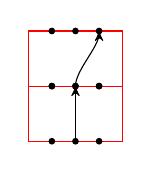
\begin{tikzpicture}[->,>=stealth']
	\tPlanar{2}{3}{2}
	\tPlanar{2}{2}{1}
	\end{tikzpicture}\end{matrix}
	=
	\begin{matrix}\atPlanar{2}{3}\end{matrix} 
	.	
	\end{equation}
	
	Notice the order of these diagrams. The multiplication of diagram $b$ to $a$ is understood as $b$ is attached to $a$ (on the top). Now we have a glimpse of a group structure of actions here. If we see these diagrams as a representation of an action threading a needle between holes, we can see the multiplication of diagram $a$ to $b$ as perform $a$ and then $b$. If we consider a product of a series of single strand diagrams, we consider the rightmost one as our ``first" action. We are playing lose with the concepts of ``actions" and ``representations" here, and we shall come back with a rigorous definition of them later. But before that we immediately see that the multiplication defined above has a loophole. 
	
	As a side note, the opposite choice is equally effective. We chose so because we chose the time to be flowing upwards. 
	
	Consider the multiplication of the following two diagrams
	\begin{equation}
	\begin{matrix}\atPlanar{2}{3}\end{matrix}
	\cdot
	\begin{matrix}\atPlanar{3}{1}\end{matrix}
	=
	\begin{matrix}
	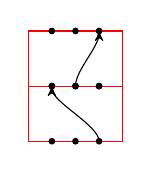
\begin{tikzpicture}[->,>=stealth']
	\tPlanar{2}{3}{2}
	\tPlanar{3}{1}{1}
	\end{tikzpicture}
	\end{matrix}
	=	?
	\end{equation}

	The multiplication gives us a broken line which we do not know how to proceed. One simple choice is to dictate that the result is simply $0$. Namely, 
	\begin{equation}
	\begin{matrix}\atPlanar{2}{3}\end{matrix}
	\cdot
	\begin{matrix}\atPlanar{3}{1}\end{matrix}
	=
	\begin{matrix}
	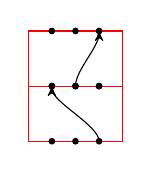
\begin{tikzpicture}[->,>=stealth']
	\tPlanar{2}{3}{2}
	\tPlanar{3}{1}{1}
	\end{tikzpicture}
	\end{matrix}
	=	0.
	\end{equation}
	
	One thing we look for a binary operation over a set is the set of the result of all possible pairs. Hence our set of results is in fact $D^{(n)}\cup \Set{0}$. If we define the multiplication of $0$ to any other diagram as $0$, we can extend the set of diagrams. And we shall use $D^{(n)}$ only to denote the extended set from now on, its cardinality $n^2+1$.
	
	This way, the product of any two elements form $D^{(n)}$ is again in $D^{(n)}$. We say that $D^{(n)}$ is \textbf{closed} under multiplication defined this way. From now on we shall use $\DD 00$ to denote $0$ and use them interchangeably whenever its convenient.
	
	You can draw some more pairs for yourself and see if you can find a nice way to calculate the result. In the appendix is the multiplication table of $n=3$, and here is the table of $n=2$.
	
	\begin{table}[ht]
		\centering	
		\begin{tabular}{|l|l|l|l|l|l|}
			\hline
			&0&
			$\begin{matrix}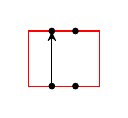
\begin{tikzpicture}[->,>=stealth']
			\bPlanar{1}{1}{1}
			\end{tikzpicture}\end{matrix}$ & 
			$\begin{matrix}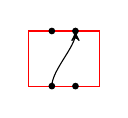
\begin{tikzpicture}[->,>=stealth']
			\bPlanar{1}{2}{1}
			\end{tikzpicture}\end{matrix}$ & 
			$\begin{matrix}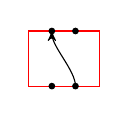
\begin{tikzpicture}[->,>=stealth']
			\bPlanar{2}{1}{1}
			\end{tikzpicture}\end{matrix}$ & 
			$\begin{matrix}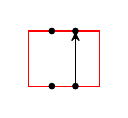
\begin{tikzpicture}[->,>=stealth']
			\bPlanar{2}{2}{1}
			\end{tikzpicture}\end{matrix}$ 
			\\\hline
			0&0&0&0&0&0\\\hline
			$\begin{matrix}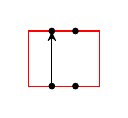
\begin{tikzpicture}[->,>=stealth']
			\bPlanar{1}{1}{1}
			\end{tikzpicture}\end{matrix}$
			& 0&
			$\begin{matrix}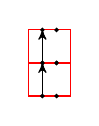
\begin{tikzpicture}[->,>=stealth',scale=0.6]
			\bPlanar{1}{1}{2}
			\bPlanar{1}{1}{1}
			\end{tikzpicture}\end{matrix}=
			\begin{matrix}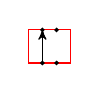
\begin{tikzpicture}[->,>=stealth',scale=0.6]
			\bPlanar{1}{1}{1}
			\end{tikzpicture}\end{matrix}$
			& 
			$\begin{matrix}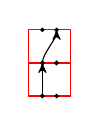
\begin{tikzpicture}[->,>=stealth',scale=0.6]
			\bPlanar{1}{2}{2}
			\bPlanar{1}{1}{1}
			\end{tikzpicture}\end{matrix}=
			\begin{matrix}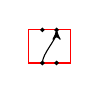
\begin{tikzpicture}[->,>=stealth',scale=0.6]
			\bPlanar{1}{2}{1}
			\end{tikzpicture}\end{matrix}$
			& 
			$\begin{matrix}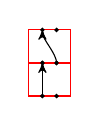
\begin{tikzpicture}[->,>=stealth',scale=0.6]
			\bPlanar{2}{1}{2}
			\bPlanar{1}{1}{1}
			\end{tikzpicture}\end{matrix}=
			0$
			& 
			$\begin{matrix}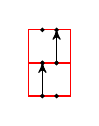
\begin{tikzpicture}[->,>=stealth',scale=0.6]
			\bPlanar{2}{2}{2}
			\bPlanar{1}{1}{1}
			\end{tikzpicture}\end{matrix}=
			0$\\ \hline
			$\begin{matrix}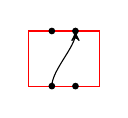
\begin{tikzpicture}[->,>=stealth']
			\bPlanar{1}{2}{1}
			\end{tikzpicture}\end{matrix}$
			& 0&
			$\begin{matrix}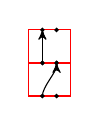
\begin{tikzpicture}[->,>=stealth',scale=0.6]
			\bPlanar{1}{1}{2}
			\bPlanar{1}{2}{1}
			\end{tikzpicture}\end{matrix}=
			0$
			& 
			$\begin{matrix}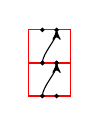
\begin{tikzpicture}[->,>=stealth',scale=0.6]
			\bPlanar{1}{2}{2}
			\bPlanar{1}{2}{1}
			\end{tikzpicture}\end{matrix}=
			0$
			& 
			$\begin{matrix}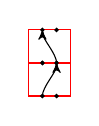
\begin{tikzpicture}[->,>=stealth',scale=0.6]
			\bPlanar{2}{1}{2}
			\bPlanar{1}{2}{1}
			\end{tikzpicture}\end{matrix}=
			\begin{matrix}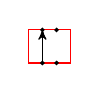
\begin{tikzpicture}[->,>=stealth',scale=0.6]
			\bPlanar{1}{1}{1}
			\end{tikzpicture}\end{matrix}$
			& 
			$\begin{matrix}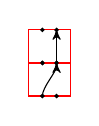
\begin{tikzpicture}[->,>=stealth',scale=0.6]
			\bPlanar{2}{2}{2}
			\bPlanar{1}{2}{1}
			\end{tikzpicture}\end{matrix}=
			\begin{matrix}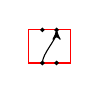
\begin{tikzpicture}[->,>=stealth',scale=0.6]
			\bPlanar{1}{2}{1}
			\end{tikzpicture}\end{matrix}$\\ \hline
			$\begin{matrix}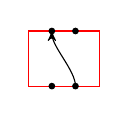
\begin{tikzpicture}[->,>=stealth']
			\bPlanar{2}{1}{1}
			\end{tikzpicture}\end{matrix}$
			& 0 &
			$\begin{matrix}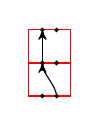
\begin{tikzpicture}[->,>=stealth',scale=0.6]
			\bPlanar{1}{1}{2}
			\bPlanar{2}{1}{1}
			\end{tikzpicture}\end{matrix}=
			\begin{matrix}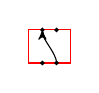
\begin{tikzpicture}[->,>=stealth',scale=0.6]
			\bPlanar{2}{1}{1}
			\end{tikzpicture}\end{matrix}$
			& 
			$\begin{matrix}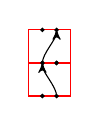
\begin{tikzpicture}[->,>=stealth',scale=0.6]
			\bPlanar{1}{2}{2}
			\bPlanar{2}{1}{1}
			\end{tikzpicture}\end{matrix}=
			\begin{matrix}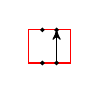
\begin{tikzpicture}[->,>=stealth',scale=0.6]
			\bPlanar{2}{2}{1}
			\end{tikzpicture}\end{matrix}$
			& 
			$\begin{matrix}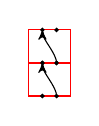
\begin{tikzpicture}[->,>=stealth',scale=0.6]
			\bPlanar{2}{1}{2}
			\bPlanar{2}{1}{1}
			\end{tikzpicture}\end{matrix}=
			0$
			& 
			$\begin{matrix}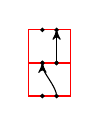
\begin{tikzpicture}[->,>=stealth',scale=0.6]
			\bPlanar{2}{2}{2}
			\bPlanar{2}{1}{1}
			\end{tikzpicture}\end{matrix}=
			0$\\ \hline
			$\begin{matrix}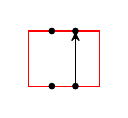
\begin{tikzpicture}[->,>=stealth']
			\bPlanar{2}{2}{1}
			\end{tikzpicture}\end{matrix}$
			& 0 &
			$\begin{matrix}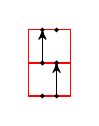
\begin{tikzpicture}[->,>=stealth',scale=0.6]
			\bPlanar{1}{1}{2}
			\bPlanar{2}{2}{1}
			\end{tikzpicture}\end{matrix}=
			0$
			& 
			$\begin{matrix}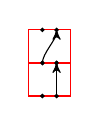
\begin{tikzpicture}[->,>=stealth',scale=0.6]
			\bPlanar{1}{2}{2}
			\bPlanar{2}{2}{1}
			\end{tikzpicture}\end{matrix}=
			0$
			& 
			$\begin{matrix}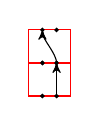
\begin{tikzpicture}[->,>=stealth',scale=0.6]
			\bPlanar{2}{1}{2}
			\bPlanar{2}{2}{1}
			\end{tikzpicture}\end{matrix}=
			\begin{matrix}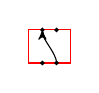
\begin{tikzpicture}[->,>=stealth',scale=0.6]
			\bPlanar{2}{1}{1}
			\end{tikzpicture}\end{matrix}$
			& 
			$\begin{matrix}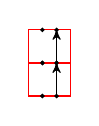
\begin{tikzpicture}[->,>=stealth',scale=0.6]
			\bPlanar{2}{2}{2}
			\bPlanar{2}{2}{1}
			\end{tikzpicture}\end{matrix}=
			\begin{matrix}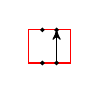
\begin{tikzpicture}[->,>=stealth',scale=0.6]
			\bPlanar{2}{2}{1}
			\end{tikzpicture}\end{matrix}$\\ \hline
		\end{tabular}
		\caption{Multiplication Table for $n=2$, multiplication rules for $0=\DD 00$ included.}
		\label{MultiplicationTable2}
	\end{table}

	We observe that the multiplication table can be summarized using the Kronecker delta. And if we use the $\DD ij$ notation (which we will be mainly using from now on), we can state the rule for multiplication of the single strand diagrams in a single line: 
	\begin{equation}
	\DD kl \cdot \DD ij = \substack{\DD kl\\ \DD ij} =\delta_{k}^{j} \DD il, \label{PlanarDiagramMultiplicationRule}
	\end{equation}
	where the $\delta_{k}^{j}$ indicates that when there is a mismatch, namely a interrupted strand, the result is $0$ diagram, which is a diagram with no strands. The Kronecker delta is written with a sub and a superscript just to look nicer for now. Here we used the scalar multiplication on the right hand side, even if that is just $0$ or $1$ multiplied by a diagram. This operation is not yet defined (how do we understand a number multiplied by an abstract diagram?). However, we will pretend that we know what it is and use it as a short hand to avoid writing down the entire multiplication table. 

	After finding out the rules, looking at the table again, the first thing we notice from the above multiplication table is that generally the multiplication does not \textbf{commute}, namely $\DD kl \cdot \DD ij \neq \DD ij  \cdot \DD kl $. 
	
	The multiplication is \textbf{associative}. Visually we can interpret that as long as we have three graphs stacked we do not care about whether we combine the lowest two or the top two.
	\begin{equation}
	\left(
	\begin{matrix}
	\atPlanar{2}{1}
	\end{matrix}\cdot
	\begin{matrix}
	\atPlanar{1}{2}
	\end{matrix}
	\right)\cdot
	\begin{matrix}
	\atPlanar{3}{1}
	\end{matrix}
	=
	\begin{matrix}
	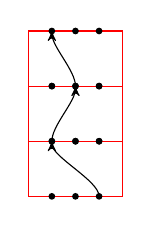
\begin{tikzpicture}[->,>=stealth']
	\tPlanar{2}{1}{3}
	\tPlanar{1}{2}{2}
	\tPlanar{3}{1}{1}
	\end{tikzpicture}
	\end{matrix}
	=
	\begin{matrix}
	\atPlanar{2}{1}
	\end{matrix}\cdot\left(
	\begin{matrix}
	\atPlanar{1}{2}
	\end{matrix}
	\cdot
	\begin{matrix}
	\atPlanar{3}{1}
	\end{matrix}\right).
	\end{equation}
	Or mathematically we have from the rule
	\begin{equation}
	\begin{aligned}
	\left(\DD ij \cdot \DD kl\right) \cdot \DD rs = \delta_{i}^{l} \DD kj\cdot  \DD rs &= \delta_{i}^{l} \delta_k^s \DD rj 
	\\
	\DD ij \cdot \left(\DD kl \cdot \DD rs\right) = \delta_k^s \DD ij \cdot \DD rl &= \delta_{i}^{l} \delta_k^s \DD rj .
	\end{aligned}
	\end{equation}
		
	Whenever we have a rule, we will be looking for special cases. Two special cases of multiplications (just like the multiplication with numbers) are the \textbf{identity} and the \textbf{absorbing element} (or the \textbf{zero element}, as $0$ ``absorbs everything to $0$"). 
	
	The identity (such as the number $1$ in kindergarten multiplication) is defined as the element which leaves any element of the set unchanged when multiplied with it. Since the multiplication does not commute, we actually have both the \textbf{left identity} and the \textbf{right identity}. 
	
	Namely $\DD ij$ is called a left identity if Eq. \eqref{leftidentity} is satisfied, and is called a right identity if Eq. \eqref{rightidentity} is satisfied. If both equations are satisfied, it is called a \textbf{two-sided identity} or just an \textbf{identity}.
	\begin{align}
	\DD kl \cdot \DD ij = \substack{\DD kl\\ \DD ij} =\delta_{k}^{j} \DD il \equiv \DD kl ,\quad \forall k,l \in \Set{0,1,2,\cdots,n} \label{leftidentity},\\
	\DD ij \cdot \DD kl = \substack{\DD ij\\ \DD kl} =\delta_{i}^{l} \DD kj \equiv \DD kl ,\quad \forall k,l \in \Set{0,1,2,\cdots,n}
	\label{rightidentity}.
	\end{align}
	
	Searching in Table \ref{MultiplicationTable2} shows that there is absolutely no identity in the set, whether it's the left identity or the right identity. $0$ is trivially the zero element.
	
	So far, we have defined a set of abstract symbols, defined a binary operation between those symbols, which is nicely summarized by Eq. \eqref{PlanarDiagramMultiplicationRule}. Optionally, we could have defined the product pairwise and have a kind of clumsy multiplication table (of size $(n+1)^2$) between the diagrams as is shown.
	
	Like the matrix multiplications, the multiplication between diagrams are non-commutative. But unlike the general matrix multiplication, it does not have an identity. But we shall see very soon how we can use a special set of matrices to ``mock" the multiplications between diagrams.
	
	\subsection{From Single Strand Diagrams to Matrix Units}
	A \textbf{matrix unit} $E_i^j$ is defined as a $n$ by $n$ matrix with the only nonzero element located at the $i^{\text{th}}$ column and $j^{\text{th}}$ row, or 
	\begin{equation}
	E_i^j = 
	\begin{pmatrix}
	& & &  \\
	& &1&  \\
	& & &  \\
	& & &  
	\end{pmatrix}, \quad \text{$1$ at and $i^\text{th}$ column and $j^\text{th}$ row; $0$ otherwise}.
	\end{equation}
	The elements in the set $\{E_i^j\}$ are called the matrix units because just like basis vectors, they give us a way to expand any matrix as
	\begin{equation}
	M=\sum_{ij} M\cdot E_i^j =\sum_{ij} M_{ij}\cdot E_i^j .
	\end{equation}
	where $M$ in the middle is a matrix and $M_{ij}$ is the matrix element, which is a number. 
	
	For example, we have for $2\times 2$ matrices we have the set of matrix elements $\Set{E_1^1,E_2^1,E_1^2,E_2^2}$ as 
	\begin{equation}
	\Set{\begin{pmatrix}
		1 & 0 \\ 0 & 0 
		\end{pmatrix},
		\begin{pmatrix}
		0 & 1 \\ 0 & 0 
		\end{pmatrix},
		\begin{pmatrix}
		0 & 0 \\ 1 & 0 
		\end{pmatrix},
		\begin{pmatrix}
		0 & 0 \\ 0 & 1 
		\end{pmatrix}}.
	\end{equation}
	Any matrix $M=\begin{pmatrix}	M_{11} & M_{12} \\ M_{21}&  M_{22} \end{pmatrix}$ can be decomposed in the following way:
	
	\begin{equation}
	\begin{aligned}
	\begin{pmatrix}
	M_{11} & M_{12} \\ M_{21} & M_{22}
	\end{pmatrix} 
	=& 
	M\cdot E_1^1 + M\cdot E_2^1 + M\cdot E_1^2 + M\cdot E_2^2 
	\\=& 
	\begin{pmatrix}	M_{11} & M_{12} \\ M_{21} & M_{22}	\end{pmatrix} 
	\begin{pmatrix}	1 & 0 \\ 0 & 0 	\end{pmatrix}+
	\begin{pmatrix}	M_{11} & M_{12} \\ M_{21} & M_{22}	\end{pmatrix} 
	\begin{pmatrix}	0 & 1 \\ 0 & 0 	\end{pmatrix}+
	\\&
	\begin{pmatrix}	M_{11} & M_{12} \\ M_{21} & M_{22}	\end{pmatrix} 
	\begin{pmatrix}	0 & 0 \\ 1 & 0 	\end{pmatrix}+
	\begin{pmatrix}	M_{11} & M_{12} \\ M_{21} & M_{22}	\end{pmatrix} 
	\begin{pmatrix}	0 & 0 \\ 0 & 1 	\end{pmatrix}
	\\=&
	M_{11}\begin{pmatrix}	1 & 0 \\ 0 & 0 	\end{pmatrix}+
	M_{12}\begin{pmatrix}	0 & 1 \\ 0 & 0 	\end{pmatrix}+
	M_{21}\begin{pmatrix}	0 & 0 \\ 1 & 0 	\end{pmatrix}+ 
	M_{22}\begin{pmatrix}	0 & 0 \\ 0 & 1 	\end{pmatrix}
	\\=& 
	\begin{pmatrix}	M_{11} & 0 \\ 0 & 0 	\end{pmatrix}+
	\begin{pmatrix}	0 & M_{12} \\ 0 & 0 	\end{pmatrix}+
	\begin{pmatrix}	0 & 0 \\ M_{21} & 0 	\end{pmatrix}+ 
	\begin{pmatrix}	0 & 0 \\ 0 & M_{22} 	\end{pmatrix},
	\end{aligned}
	\end{equation}
	which is evident when we get to the final result.
	
	The multiplication between the matrix units are by definition
	\begin{equation}
	\begin{aligned}
	(E_i^j \cdot E_k^l )_{ac}
	=& \sum_{b=1}^n (E_i^j)_{ab} (E_k^l)_{bc}\\
	=& (E_i^j)_{ai} (E_k^l)_{lc} \delta_{il}\\
	=& \delta_{aj} \delta_{kc} \delta_{il},
	\end{aligned}
	\label{MatrixUnitsMultiplicationRule}
	\end{equation}
	hence the only nonzero element of the result $E_i^j \cdot E_k^l$ is when $a=j$, $k=c$ and $i=l$. That is to say, the result is just
	\begin{equation}
	E_i^j \cdot E_k^l=\delta_{i}^{l} E_k^j.
	\end{equation}
	Fortunately we do not need to write down a multiplication table for the matrix units since we are well versed in matrix multiplications already and have deduced the result. However you can still check the result by writing down some examples such as 
	\begin{equation}
	\begin{aligned}
	E_1^1 \cdot E_2^1 &= 	
	\begin{pmatrix} 1 & 0 \\ 0 & 0 	\end{pmatrix}\cdot 
	\begin{pmatrix}	0 & 1 \\ 0 & 0 	\end{pmatrix}
	=\begin{pmatrix}	0 & 1 \\ 0 & 0 	\end{pmatrix}
	=E_2^1
	\\
	E_1^1 \cdot E_1^2 &= 	
	\begin{pmatrix} 1 & 0 \\ 0 & 0 	\end{pmatrix}\cdot 
	\begin{pmatrix}	0 & 0 \\ 1 & 0 	\end{pmatrix}
	=\begin{pmatrix}	0 & 0 \\ 0 & 0 	\end{pmatrix}
	=: E_0^0.
	\end{aligned}
	\end{equation}
	where we define $E_0^0$ as the matrix with $0$ at all entries. We shall denote $\Set{E_i^j}\cup\Set{0} $ as $E^{(n)}$.
	
	Now that we have established the multiplication rule between matrix units, we can start addressing the resemblance between Eq. \eqref{PlanarDiagramMultiplicationRule} and Eq. \eqref{MatrixUnitsMultiplicationRule}, both of them are listed below:
	\begin{align*}
	\DD ij\cdot \DD kl & =\delta_{kj} \DD il,\\
	E_i^j \cdot E_k^l &= \delta^j_k E_i^l.
	\end{align*}
	If we make the correspondence 
	\begin{equation}
	\DD ij \leftrightarrow E_i^j, \text{especially}\quad \DD 00 \leftrightarrow E_0^0,
	\end{equation}
	we will have a one-to-one map from single strand diagrams to matrix units that preserves the multiplication rule. 
	
	The above correspondence is actually called an \textbf{homomorphism} between $E^{(n)}$ and $D^{(n)}$. A homomorphism is a map $f$ from a set $E^{(n)}$ to $D^{(n)}$, commonly denoted as 
	\begin{equation}
	f: \, E^{(n)} \rightarrow D^{(n)}; \quad E_i^j \mapsto f(E_i^j) = D^{(n)}, E_0^0 \mapsto f(E_0^0)= \DD 00,
	\end{equation}
	where the symbol $\mapsto$ reads ``maps to". The defining feature of a homomorphism is that it preserves the structure, namely 
	\begin{equation}
	\begin{aligned}
	f(E_i^j)\cdot f(E_k^l) =& f(E_i^j \cdot E_k^l)\\
	\DD ij \cdot \DD kl =& f(\delta_i^l  E_k^j)\\
	\delta_i^l \DD kj =& \delta_i^l f(E_k^j) \\
	=&\delta_i^l \DD kj 
	\end{aligned}
	\end{equation}
	
	We have the map from $E_i^j$ to $\DD ij$ and its inverse are both homomorphisms. Hence the map is called an \textbf{isomorphism}. In many cases, and two structures that are isomorphic can be considered as virtually the same. 	
	
	We can call the above isomorphism a \textbf{matrix representation} of the original set of diagrams. We will have further discussion of what representation means in later sections. For now, it serves our purposes to simply state that studying the diagrams under multiplication is ``equivalent" to studying the matrix units under matrix multiplications.
	
	\subsection{Matrix Semi-groups}
	Whenever we have set with a structure (some operation) defined, there is a name for it. There is an hierarchy in the names. One branch is that first we have the set $S$. If we define a binary operation $\cdot$ on the set such that the set is \textbf{closed under finite composition}, we say that the set along with this binary operation is a \textbf{magma}, denoted as $(S, \cdot)$. If the binary operation is associative, it is called a \textbf{semi-group}. Further, if there is at least one identity, and a unique inverse for each element, we call the structure $(S, \cdot)$ a \textbf{group}. The concept of groups will be discussed later.
	
	Notice that we emphasize on the closure is only under finite composition. Normally we will just say that $S$ is closed under some binary operation, where the closure under infinite composition is \textit{never} implied. The statement hints us  that there are cases when you apply an binary operation on a group, you might end up outside the group even if the group is ``closed" under it. To name a few examples, 
	\begin{itemize}
		\item The rational numbers $\mathbb Q$ are closed under addition. When you add two rational numbers, you will have yet another rational number. The problem arises when you have infinite amount of rational numbers. The famous example being 
		\begin{equation*}
		\sum_{n=1}^\infty \frac{1}{n^2} = \frac{\pi^2}{6} \notin \mathbb Q.
		\end{equation*} 
		\item The permutation group of two elements consist of two operations: either we exchange the two elements, denoted as $\sigma$, or we do nothing to them, denoted as $e$. If we ignore the identity and inverse of the group and just treat it just as a semi-group, The set $\Set{\sigma,e}$ is definitely closed. The statement is evident since there are only two possible ways to arrange these two elements. Written explicitly, we have
		\begin{equation*}
		\sigma^n=\begin{cases}
		\sigma, \quad n \text{ odd}\\
		e,\quad n \text{ even}
		\end{cases}.
		\end{equation*}
		But we no not know $\lim_{n\rightarrow \infty} \sigma^n$. The series does not converge at all. The infinite composition is not defined here.
	\end{itemize}

	The moral of the above examples is that when we are dealing with consecutive operations (and we will), we have to be careful that we do not go to infinity so we know that the result is meaningful.	
		
	Now it's evident that the matrix elements along with $0$ under matrix multiplication
	\begin{equation}
	E_i^j \cdot E_k^l = \delta^j_k E_i^l
	\end{equation}
	is closed. And the operation we know and love from matrix algebra is associative. But we do not have an identity, let alone an inverse. That makes our set of matrix units along with $0$ a semi-group. The same is true for the set of diagrams $(D^{(n)},\cdot )$.
	
	\subsection{Subsets of the semi-groups}
	Now we have known that the diagrams form a semi-group and we have a nice way to symbolize these diagrams using matrix elements, we will study the internal sub-structures of the diagram semi-groups. 
	
	Look at the multiplication table again, we notice something interesting here:
	\begin{table}[ht]
		\centering	
		\begin{tabular}{|l|l|l|l|l|l|}
			\hline
			&\cellcolor{SpringGreen}0&
			\cellcolor{Aquamarine}
			$\begin{matrix}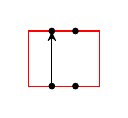
\begin{tikzpicture}[->,>=stealth']
			\bPlanar{1}{1}{1}
			\end{tikzpicture}\end{matrix}$ & 
			\cellcolor{Aquamarine}
			$\begin{matrix}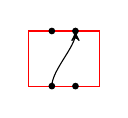
\begin{tikzpicture}[->,>=stealth']
			\bPlanar{1}{2}{1}
			\end{tikzpicture}\end{matrix}$ &
			\cellcolor{Dandelion}  
			$\begin{matrix}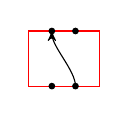
\begin{tikzpicture}[->,>=stealth']
			\bPlanar{2}{1}{1}
			\end{tikzpicture}\end{matrix}$ &
			\cellcolor{Dandelion} 
			$\begin{matrix}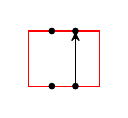
\begin{tikzpicture}[->,>=stealth']
			\bPlanar{2}{2}{1}
			\end{tikzpicture}\end{matrix}$ 
			\\\hline
			\cellcolor{SpringGreen}0&\cellcolor{SpringGreen}0&0&0&0&0\\\hline
			\cellcolor{Aquamarine}
			$\begin{matrix}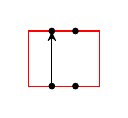
\begin{tikzpicture}[->,>=stealth']
			\bPlanar{1}{1}{1}
			\end{tikzpicture}\end{matrix}$
			&0
			&\cellcolor{Aquamarine}
			$\begin{matrix}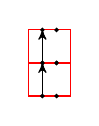
\begin{tikzpicture}[->,>=stealth',scale=0.6]
			\bPlanar{1}{1}{2}
			\bPlanar{1}{1}{1}
			\end{tikzpicture}\end{matrix}=
			\begin{matrix}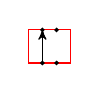
\begin{tikzpicture}[->,>=stealth',scale=0.6]
			\bPlanar{1}{1}{1}
			\end{tikzpicture}\end{matrix}$
			&\cellcolor{Aquamarine}
			$\begin{matrix}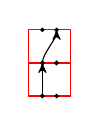
\begin{tikzpicture}[->,>=stealth',scale=0.6]
			\bPlanar{1}{2}{2}
			\bPlanar{1}{1}{1}
			\end{tikzpicture}\end{matrix}=
			\begin{matrix}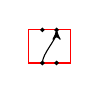
\begin{tikzpicture}[->,>=stealth',scale=0.6]
			\bPlanar{1}{2}{1}
			\end{tikzpicture}\end{matrix}$
			& 
			$\begin{matrix}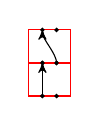
\begin{tikzpicture}[->,>=stealth',scale=0.6]
			\bPlanar{2}{1}{2}
			\bPlanar{1}{1}{1}
			\end{tikzpicture}\end{matrix}=
			0$
			& 
			$\begin{matrix}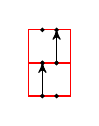
\begin{tikzpicture}[->,>=stealth',scale=0.6]
			\bPlanar{2}{2}{2}
			\bPlanar{1}{1}{1}
			\end{tikzpicture}\end{matrix}=
			0$\\ \hline
			\cellcolor{Aquamarine}
			$\begin{matrix}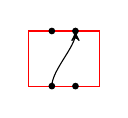
\begin{tikzpicture}[->,>=stealth']
			\bPlanar{1}{2}{1}
			\end{tikzpicture}\end{matrix}$
			&0
			&\cellcolor{Aquamarine}
			$\begin{matrix}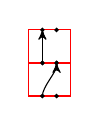
\begin{tikzpicture}[->,>=stealth',scale=0.6]
			\bPlanar{1}{1}{2}
			\bPlanar{1}{2}{1}
			\end{tikzpicture}\end{matrix}=
			0$
			&\cellcolor{Aquamarine}
			$\begin{matrix}\begin{tikzpicture}[->,>=stealth',scale=0.6]
			\bPlanar{1}{2}{2}
			\bPlanar{1}{2}{1}
			\end{tikzpicture}\end{matrix}=
			0$
			& 
			$\begin{matrix}\begin{tikzpicture}[->,>=stealth',scale=0.6]
			\bPlanar{2}{1}{2}
			\bPlanar{1}{2}{1}
			\end{tikzpicture}\end{matrix}=
			\begin{matrix}\begin{tikzpicture}[->,>=stealth',scale=0.6]
			\bPlanar{1}{1}{1}
			\end{tikzpicture}\end{matrix}$
			& 
			$\begin{matrix}\begin{tikzpicture}[->,>=stealth',scale=0.6]
			\bPlanar{2}{2}{2}
			\bPlanar{1}{2}{1}
			\end{tikzpicture}\end{matrix}=
			\begin{matrix}\begin{tikzpicture}[->,>=stealth',scale=0.6]
			\bPlanar{1}{2}{1}
			\end{tikzpicture}\end{matrix}$\\ \hline
			\cellcolor{Dandelion}
			$\begin{matrix}\begin{tikzpicture}[->,>=stealth']
			\bPlanar{2}{1}{1}
			\end{tikzpicture}\end{matrix}$
			&0 & 
			$\begin{matrix}\begin{tikzpicture}[->,>=stealth',scale=0.6]
			\bPlanar{1}{1}{2}
			\bPlanar{2}{1}{1}
			\end{tikzpicture}\end{matrix}=
			\begin{matrix}\begin{tikzpicture}[->,>=stealth',scale=0.6]
			\bPlanar{2}{1}{1}
			\end{tikzpicture}\end{matrix}$
			& 
			$\begin{matrix}\begin{tikzpicture}[->,>=stealth',scale=0.6]
			\bPlanar{1}{2}{2}
			\bPlanar{2}{1}{1}
			\end{tikzpicture}\end{matrix}=
			\begin{matrix}\begin{tikzpicture}[->,>=stealth',scale=0.6]
			\bPlanar{2}{2}{1}
			\end{tikzpicture}\end{matrix}$
			&\cellcolor{Dandelion}
			$\begin{matrix}\begin{tikzpicture}[->,>=stealth',scale=0.6]
			\bPlanar{2}{1}{2}
			\bPlanar{2}{1}{1}
			\end{tikzpicture}\end{matrix}=
			0$
			&\cellcolor{Dandelion}
			$\begin{matrix}\begin{tikzpicture}[->,>=stealth',scale=0.6]
			\bPlanar{2}{2}{2}
			\bPlanar{2}{1}{1}
			\end{tikzpicture}\end{matrix}=
			0$\\ \hline
			\cellcolor{Dandelion}
			$\begin{matrix}\begin{tikzpicture}[->,>=stealth']
			\bPlanar{2}{2}{1}
			\end{tikzpicture}\end{matrix}$
			& 0&
			$\begin{matrix}\begin{tikzpicture}[->,>=stealth',scale=0.6]
			\bPlanar{1}{1}{2}
			\bPlanar{2}{2}{1}
			\end{tikzpicture}\end{matrix}=
			0$
			& 
			$\begin{matrix}\begin{tikzpicture}[->,>=stealth',scale=0.6]
			\bPlanar{1}{2}{2}
			\bPlanar{2}{2}{1}
			\end{tikzpicture}\end{matrix}=
			0$
			&\cellcolor{Dandelion}
			$\begin{matrix}\begin{tikzpicture}[->,>=stealth',scale=0.6]
			\bPlanar{2}{1}{2}
			\bPlanar{2}{2}{1}
			\end{tikzpicture}\end{matrix}=
			\begin{matrix}\begin{tikzpicture}[->,>=stealth',scale=0.6]
			\bPlanar{2}{1}{1}
			\end{tikzpicture}\end{matrix}$
			&\cellcolor{Dandelion}
			$\begin{matrix}\begin{tikzpicture}[->,>=stealth',scale=0.6]
			\bPlanar{2}{2}{2}
			\bPlanar{2}{2}{1}
			\end{tikzpicture}\end{matrix}=
			\begin{matrix}\begin{tikzpicture}[->,>=stealth',scale=0.6]
			\bPlanar{2}{2}{1}
			\end{tikzpicture}\end{matrix}$\\ \hline
		\end{tabular}
		\caption{Multiplication Table for $n=2$. Subsections are highlighted.}
		\label{MultiplicationTable2LeftHighlighted}
	\end{table}
	
	The graphs highlighted with the same color (with $0$) is closed under the multiplication as well. Take the set $L_1=\Set{0,
	\begin{matrix}\begin{tikzpicture}[->,>=stealth']
	\bPlanar{1}{1}{1}
	\end{tikzpicture}\end{matrix}, 
	\begin{matrix}\begin{tikzpicture}[->,>=stealth']
	\bPlanar{1}{2}{1}
	\end{tikzpicture}\end{matrix} }$ for example. If we are only allowed to use elements from this set, we will never have a diagram whose strand starts from the bottom right dot. The same is true for the set $L_2=\Set{0,
	\begin{matrix}\begin{tikzpicture}[->,>=stealth']
	\bPlanar{2}{1}{1}
	\end{tikzpicture}\end{matrix}, 
	\begin{matrix}\begin{tikzpicture}[->,>=stealth']
	\bPlanar{2}{2}{1}
	\end{tikzpicture}\end{matrix} }$. It's easy to check that $L_1$ and $L_2$ are indeed semi-groups. They are the subsets of the semi-group $D^{(n)}$ equipped with the same multiplication rule. They are called the \textbf{sub-semi-groups} of $D^{(n)}$. 

	That being said, we further find out that $L_1$ and $L_2$ are actually attractors of $D^{(n)}$. Since multiplying a graph $D$ from the left to another graph $D'$ does not alter the bottom dot of graph $D'$. We will use the following notations to better state the idea, 
	\begin{align*}
	D \cdot L &= \Set{D\cdot D' | D'\in L},\, D\in D^{(n)}\\
	D^{(n)}\cdot L &= \Set{D\cdot D' | D\in D^{(n)},\,D'\in L},
	\end{align*}
	and the above statement ends up as $D^{(n)}L_i =L_i$, $i=1,2,\cdots,n$. Later we will see that these sub-semi-groups once equipped with other structures are actually \textbf{left ideals}. 
	
	It's natural for us to generalize the above concepts to multiplications on the right, and define two other sets $R_1$ and $R_2$, as is evident from Table. \ref{MultiplicationTable2RightHighlighted}. Similarly any multiplication from the right cannot alter the top dot of the left diagram, so we have $R_i$ are sub-semi-groups and they act like absorbers or attractors in the entire semi-group $R_i D^{(n)}=R_i$, $i=1,2,\cdots,n$. We see the role of non-commutative multiplication here that $R_i\neq L_i$. The $R_i$'s are similar to \textbf{right ideals}. 
	
	\begin{table}[ht]
		\centering	
		\begin{tabular}{|l|l|l|l|l|l|}
			\hline
			&\cellcolor{SpringGreen}0&
			\cellcolor{Aquamarine}
			$\begin{matrix}\begin{tikzpicture}[->,>=stealth']
			\bPlanar{1}{1}{1}
			\end{tikzpicture}\end{matrix}$ & 
			\cellcolor{Dandelion}
			$\begin{matrix}\begin{tikzpicture}[->,>=stealth']
			\bPlanar{1}{2}{1}
			\end{tikzpicture}\end{matrix}$ &
			\cellcolor{Aquamarine}  
			$\begin{matrix}\begin{tikzpicture}[->,>=stealth']
			\bPlanar{2}{1}{1}
			\end{tikzpicture}\end{matrix}$ &
			\cellcolor{Dandelion} 
			$\begin{matrix}\begin{tikzpicture}[->,>=stealth']
			\bPlanar{2}{2}{1}
			\end{tikzpicture}\end{matrix}$ 
			\\\hline
			\cellcolor{SpringGreen}0&\cellcolor{SpringGreen}0&0&0&0&0\\\hline
			\cellcolor{Aquamarine}
			$\begin{matrix}\begin{tikzpicture}[->,>=stealth']
			\bPlanar{1}{1}{1}
			\end{tikzpicture}\end{matrix}$
			&0
			& \cellcolor{Aquamarine}
			$\begin{matrix}\begin{tikzpicture}[->,>=stealth',scale=0.6]
			\bPlanar{1}{1}{2}
			\bPlanar{1}{1}{1}
			\end{tikzpicture}\end{matrix}=
			\begin{matrix}\begin{tikzpicture}[->,>=stealth',scale=0.6]
			\bPlanar{1}{1}{1}
			\end{tikzpicture}\end{matrix}$
			&
			$\begin{matrix}\begin{tikzpicture}[->,>=stealth',scale=0.6]
			\bPlanar{1}{2}{2}
			\bPlanar{1}{1}{1}
			\end{tikzpicture}\end{matrix}=
			\begin{matrix}\begin{tikzpicture}[->,>=stealth',scale=0.6]
			\bPlanar{1}{2}{1}
			\end{tikzpicture}\end{matrix}$
			& \cellcolor{Aquamarine}
			$\begin{matrix}\begin{tikzpicture}[->,>=stealth',scale=0.6]
			\bPlanar{2}{1}{2}
			\bPlanar{1}{1}{1}
			\end{tikzpicture}\end{matrix}=
			0$
			& 
			$\begin{matrix}\begin{tikzpicture}[->,>=stealth',scale=0.6]
			\bPlanar{2}{2}{2}
			\bPlanar{1}{1}{1}
			\end{tikzpicture}\end{matrix}=
			0$\\ \hline
			\cellcolor{Dandelion} 
			$\begin{matrix}\begin{tikzpicture}[->,>=stealth']
			\bPlanar{1}{2}{1}
			\end{tikzpicture}\end{matrix}$
			&0
			& 
			$\begin{matrix}\begin{tikzpicture}[->,>=stealth',scale=0.6]
			\bPlanar{1}{1}{2}
			\bPlanar{1}{2}{1}
			\end{tikzpicture}\end{matrix}=
			0$
			&  \cellcolor{Dandelion} 
			$\begin{matrix}\begin{tikzpicture}[->,>=stealth',scale=0.6]
			\bPlanar{1}{2}{2}
			\bPlanar{1}{2}{1}
			\end{tikzpicture}\end{matrix}=
			0$
			& 
			$\begin{matrix}\begin{tikzpicture}[->,>=stealth',scale=0.6]
			\bPlanar{2}{1}{2}
			\bPlanar{1}{2}{1}
			\end{tikzpicture}\end{matrix}=
			\begin{matrix}\begin{tikzpicture}[->,>=stealth',scale=0.6]
			\bPlanar{1}{1}{1}
			\end{tikzpicture}\end{matrix}$
			&  \cellcolor{Dandelion} 
			$\begin{matrix}\begin{tikzpicture}[->,>=stealth',scale=0.6]
			\bPlanar{2}{2}{2}
			\bPlanar{1}{2}{1}
			\end{tikzpicture}\end{matrix}=
			\begin{matrix}\begin{tikzpicture}[->,>=stealth',scale=0.6]
			\bPlanar{1}{2}{1}
			\end{tikzpicture}\end{matrix}$\\ \hline
			\cellcolor{Aquamarine}
			$\begin{matrix}\begin{tikzpicture}[->,>=stealth']
			\bPlanar{2}{1}{1}
			\end{tikzpicture}\end{matrix}$
			&0 & \cellcolor{Aquamarine}
			$\begin{matrix}\begin{tikzpicture}[->,>=stealth',scale=0.6]
			\bPlanar{1}{1}{2}
			\bPlanar{2}{1}{1}
			\end{tikzpicture}\end{matrix}=
			\begin{matrix}\begin{tikzpicture}[->,>=stealth',scale=0.6]
			\bPlanar{2}{1}{1}
			\end{tikzpicture}\end{matrix}$
			& 
			$\begin{matrix}\begin{tikzpicture}[->,>=stealth',scale=0.6]
			\bPlanar{1}{2}{2}
			\bPlanar{2}{1}{1}
			\end{tikzpicture}\end{matrix}=
			\begin{matrix}\begin{tikzpicture}[->,>=stealth',scale=0.6]
			\bPlanar{2}{2}{1}
			\end{tikzpicture}\end{matrix}$
			& \cellcolor{Aquamarine}
			$\begin{matrix}\begin{tikzpicture}[->,>=stealth',scale=0.6]
			\bPlanar{2}{1}{2}
			\bPlanar{2}{1}{1}
			\end{tikzpicture}\end{matrix}=
			0$
			&
			$\begin{matrix}\begin{tikzpicture}[->,>=stealth',scale=0.6]
			\bPlanar{2}{2}{2}
			\bPlanar{2}{1}{1}
			\end{tikzpicture}\end{matrix}=
			0$\\ \hline
			\cellcolor{Dandelion}
			$\begin{matrix}\begin{tikzpicture}[->,>=stealth']
			\bPlanar{2}{2}{1}
			\end{tikzpicture}\end{matrix}$
			& 0&
			$\begin{matrix}\begin{tikzpicture}[->,>=stealth',scale=0.6]
			\bPlanar{1}{1}{2}
			\bPlanar{2}{2}{1}
			\end{tikzpicture}\end{matrix}=
			0$
			&  \cellcolor{Dandelion}
			$\begin{matrix}\begin{tikzpicture}[->,>=stealth',scale=0.6]
			\bPlanar{1}{2}{2}
			\bPlanar{2}{2}{1}
			\end{tikzpicture}\end{matrix}=
			0$
			&
			$\begin{matrix}\begin{tikzpicture}[->,>=stealth',scale=0.6]
			\bPlanar{2}{1}{2}
			\bPlanar{2}{2}{1}
			\end{tikzpicture}\end{matrix}=
			\begin{matrix}\begin{tikzpicture}[->,>=stealth',scale=0.6]
			\bPlanar{2}{1}{1}
			\end{tikzpicture}\end{matrix}$
			& \cellcolor{Dandelion}
			$\begin{matrix}\begin{tikzpicture}[->,>=stealth',scale=0.6]
			\bPlanar{2}{2}{2}
			\bPlanar{2}{2}{1}
			\end{tikzpicture}\end{matrix}=
			\begin{matrix}\begin{tikzpicture}[->,>=stealth',scale=0.6]
			\bPlanar{2}{2}{1}
			\end{tikzpicture}\end{matrix}$\\ \hline
		\end{tabular}
		\caption{Multiplication Table for $n=2$. Subsections are highlighted.}
		\label{MultiplicationTable2RightHighlighted}
	\end{table}
	
	Finally, we see that the sub-semi-group $I \subseteq D^{(n)}$ which is the absorber from both sides 
	\begin{align}
	I \cdot D^{(n)} = D^{(n)} \cdot I= I
	\end{align}
	can only be $\Set{\DD 00}$ and $D^{(n)}$ itself.
	
	\subsection{Single Strand Diagram Additions}
		
	We have defined a somewhat intuitive binary operation on the set of diagrams, namely the multiplication by stacking on top. We ended up with a semi-group. Now we will define another type of binary operation on the set of diagrams, called the addition. 
	\begin{equation*}
	\begin{matrix}\atPlanar{1}{1}\end{matrix}
	+
	\begin{matrix}\atPlanar{1}{1}\end{matrix}
	\, ,\quad
	\begin{matrix}\atPlanar{1}{2}\end{matrix}
	+
	\begin{matrix}\atPlanar{2}{3}\end{matrix}
	\end{equation*}	
	One way to see the summation is the following
	\begin{equation}
	\begin{matrix}\atPlanar{1}{2}\end{matrix}
	+
	\begin{matrix}\atPlanar{2}{3}\end{matrix}
	=
	\begin{matrix}
	\begin{tikzpicture}[->,>=stealth']
	\draw[color=red] (0,0) rectangle (1.2,0.7);
	\filldraw (0.3,0) circle [radius=1pt];
	\filldraw (0.6,0) circle [radius=1pt];
	\filldraw (0.9,0) circle [radius=1pt];
	\filldraw (0.3,0.7) circle [radius=1pt];
	\filldraw (0.6,0.7) circle [radius=1pt];
	\filldraw (0.9,0.7) circle [radius=1pt];
	\draw (0.3*1,0) .. controls +(0,0.2) and +(0,-0.2) .. (0.3*2,0.7);
	\draw (0.3*2,0) .. controls +(0,0.2) and +(0,-0.2) .. (0.3*3,0.7);
	\end{tikzpicture}
	\end{matrix}.
	\end{equation}
	Of course such notation will pose a number of problems in the foreseeable future. When we go to consecutive additions, weird things as intercepting strands, multiple strands will arise. Also when we try to apply multiplications between sums of diagrams, we will have to deal with diagrams that looks like this.
	\begin{equation}
	\begin{matrix}
	\begin{tikzpicture}[->,>=stealth']
	\draw[color=red] (0,0) rectangle (1.2,0.7);
	\filldraw (0.3,0) circle [radius=1pt];
	\filldraw (0.6,0) circle [radius=1pt];
	\filldraw (0.9,0) circle [radius=1pt];
	\filldraw (0.3,0.7) circle [radius=1pt];
	\filldraw (0.6,0.7) circle [radius=1pt];
	\filldraw (0.9,0.7) circle [radius=1pt];
	\draw (0.3*1,0) .. controls +(0,0.2) and +(0,-0.2) .. (0.3*2,0.7);
	\draw (0.3*3,0) .. controls +(0,0.2) and +(0,-0.2) .. (0.3*1,0.7);
	\draw (0.3*3,0) .. controls +(0,0.2) and +(0,-0.2) .. (0.3*3,0.7);
	\node at (0.4,0.1) {\scriptsize$a$};
	\node at (0.2,0.5) {\scriptsize$b$};
	\node at (1,0.5) {\scriptsize$c$};
	\end{tikzpicture}
	\end{matrix}, 
	\end{equation}
	where $a$, $b$ and $c$ are numbers showing the multiplicity of strands. 
	
	Granted, we can device a few rules to work with the above multi-strand diagrams, the notation is still a nice way to visualize the summation, and we might come back to this type of visualization later. But here let us conclude that the above rule provides us with a one-to-one correspondence between a summation of an unordered sequence and a ``tangled" strands diagram. 
	
	However, if we simply consider the addition expression itself
	\begin{equation*}
	\begin{aligned}
	\begin{matrix}\atPlanar{1}{1}\end{matrix}
	+
	\begin{matrix}\atPlanar{1}{1}\end{matrix}\,, \quad 
	\begin{matrix}\atPlanar{1}{2}\end{matrix}
	+
	\begin{matrix}\atPlanar{2}{3}\end{matrix}\,,\cdots
	\end{aligned}
	\end{equation*}
	and collect the common terms just to write the answers trivially, 
	\begin{equation}
	\begin{aligned}
	\begin{matrix}\atPlanar{1}{1}\end{matrix}
	+
	\begin{matrix}\atPlanar{1}{1}\end{matrix}
	&=2 \times \begin{matrix}\atPlanar{1}{1}\end{matrix}\,,\qquad 
	\begin{matrix}\atPlanar{1}{2}\end{matrix}
	+
	\begin{matrix}\atPlanar{2}{3}\end{matrix}
	&=\begin{matrix}\atPlanar{1}{2}\end{matrix}
	+
	\begin{matrix}\atPlanar{2}{3}\end{matrix},\cdots
	\end{aligned}
	\end{equation}
	we actually have the better answer. 
	
	The reason is as follows. If we strictly treat these diagrams as abstract objects and insist attaching no meanings to them whatsoever, the only way for us to define an addition is exactly above.	Consider the ``addition" we did in kindergarten, what do we get when we put together one apple and one apple and one apple and one lemon and one lemon? Exactly the collection of three apples and two lemons! As there is no way to combine an apple with a lemon, we will simply write them as they are.
	\begin{equation*}
	\begin{matrix}
	\begin{tikzpicture}[every node/.style={scale=0.4}]
	\draw (0,0) pic {apple};
	\end{tikzpicture}
	\end{matrix}
	+
	\begin{matrix}
	\begin{tikzpicture}[every node/.style={scale=0.4}]
	\draw (0,0) pic {apple};
	\end{tikzpicture}
	\end{matrix}
	+
	\begin{matrix}
	\begin{tikzpicture}[every node/.style={scale=0.4}]
	\draw (0,0) pic {apple};
	\end{tikzpicture}
	\end{matrix}
	+
	\begin{matrix}
	\begin{tikzpicture}[every node/.style={scale=0.4}]
	\draw (0,0) pic {lemon};
	\end{tikzpicture}
	\end{matrix}
	+
	\begin{matrix}
	\begin{tikzpicture}[every node/.style={scale=0.4}]
	\draw (0,0) pic {lemon};
	\end{tikzpicture}
	\end{matrix}
	=
	\begin{matrix}
	\begin{tikzpicture}[every node/.style={scale=0.4}]
	\draw (0.7,0) pic {apple};
	\draw (0.35,0) pic {apple};
	\draw (0,0) pic {apple};
	\end{tikzpicture}
	\end{matrix}
	+
	\begin{matrix}
	\begin{tikzpicture}[every node/.style={scale=0.4}]
	\draw (0.35,0) pic {lemon};
	\draw (0,0) pic {lemon};
	\end{tikzpicture}
	\end{matrix}
	=
	3\times
	\begin{matrix}
	\begin{tikzpicture}[every node/.style={scale=0.4}]
	\draw (0,0) pic {apple};
	\end{tikzpicture}
	\end{matrix}
	+2\times
	\begin{matrix}
	\begin{tikzpicture}[every node/.style={scale=0.4}]
	\draw (0,0) pic {lemon};
	\end{tikzpicture}
	\end{matrix}.
	\end{equation*}
	
	Hence from now on we will define the addition between two diagrams as we would do to any abstract objects: by collecting the identical terms and listing different terms ``as they are". 
	
	Think about the action of collecting the terms. What do we mean when we write down the expression $3\times \begin{matrix}\begin{tikzpicture}[every node/.style={scale=0.2}]
	\draw (0,0) pic {apple};\end{tikzpicture}\end{matrix}$? We only have multiplication between numbers, not a number and an object. We are indeed using the expression as a shorthand just to denote collection of $3$ apples. This type of product is actually a different type of operation called the \textbf{scalar product}. (By the way the elementary school's way to teaching multiplication is indeed a hint to the concept of \textbf{vector spaces} and eventually \textbf{fields}.) 
	
	Instead of positive integer numbers of apples, we can also have fractions of apples. And if we consider the action of taking away apples, we can have negative apples as well. Following this train of thought, we can easily generalize the scalars from natural numbers to complex numbers. Applying the idea to single strand diagrams, we consider the set $\mathbf D^{(n)}$ (\textit{recall the semi-group is denoted in italicized text as} $D^{(n)}$) together with addition and scalar multiplication, defined as
	\begin{equation*}
	\mathbf D^{(n)} = \Set{A = \alpha_{00}\times \DD 00 + \sum_{i,j=1}^n \alpha_{ij} \times \DD ij | \alpha_{00},\,\alpha_{ij}\in \mathbb F,\, \DD ij \in D^{(n)}},\quad \mathbb F =\mathbb N, \mathbb C, \dots
	\end{equation*}
	
	The addition of $\DD 00$ is worth noting. Observe that multiples of the empty strand diagrams is still an empty strand, hence $ c\times \DD 00 = 0$, $c\in \mathbb F$. We can happily lose the term.
	\begin{equation}
	\mathbf D^{(n)} = \Set{A = \sum_{i,j=1}^n \alpha_{ij} \times \DD ij | \alpha_{ij}\in \mathbb F,\, \DD ij \in D^{(n)}},\quad \mathbb F =\mathbb N, \mathbb C, \dots
	\end{equation}
	
	On this set we define two operations. 
	\begin{enumerate}[leftmargin=2\parindent]
	\item Addition $+$ between two elements in $\mathbf D^{(n)}$ expressed as map:
	\begin{equation}
	+: (\mathbf D^{(n)} , \mathbf D^{(n)}) \rightarrow \mathbf D^{(n)},\quad  A+A' \mapsto A+A' \in \mathbf D^{(n)}.
	\end{equation}
	\item Scalar product $ \times$ which involves a number from field $\mathbb F$ and an element from $\mathbf D^{(n)}$, and the result is still in $\mathbf D^{(n)}$. The scalar product is again a map: 
	\begin{equation}
	\times: (\mathbb F , \mathbf D^{(n)}) \rightarrow \mathbf D^{(n)};\quad (a,A)\mapsto a\times A.
	\end{equation}
	\end{enumerate}
	It's evident that the set $\mathbf D^{(n)}$ is closed under addition and scalar multiplication. We will denote the set together with addition and scalar product as $(\mathbf D^{(n)}, +, \times, \mathbb F)$. 
	
	\subsection{Single Strand Diagram Vector Spaces}
	
	Now that we have a structure $(\mathbf D^{(n)}, +, \times, \mathbb F)$. We can check that it satisfies the following requirements:
	\begin{enumerate}[leftmargin=2\parindent]
		\item Associativity of addition: $(A+B)+C = A+(B+C)$.
		\item Commutativity of addition: $A+B=B+A$.
		\item Identity element of addition: $\exists 0 \in \mathbf D^{(n)}$ such that $0+A=A$, for all $A\in \mathbf D^{(n)}$. 
		\item Inverse elements of addition: For every $A\in \mathbf D^{(n)}$, there exists an element $-A\in \mathbf D^{(n)}$ called the additive inverse of $A$, such that $A+(-A)= 0$. 
		\item Compatibility of scalar multiplication with field multiplication:  $a\times (b\times A) = (a\times b)\times A$.
		\item Identity element of scalar multiplication: $1\times A = A$, where 1 denotes the multiplicative identity in F.
		\item Distributivity of scalar multiplication with respect to vector addition: $a\times (A + B) = a\times A + a\times B$.
		\item Distributivity of scalar multiplication with respect to field addition: $(a + b)\times A = a\times A + b\times A$.
	\end{enumerate}
	And this makes $(\mathbf D^{(n)}, +, \times, \mathbb F)$ a \textbf{vector space over a field $\mathbb F$}. We will use $(\mathbf D^{(n)}, +)$ to imply the vector space where the scalar multiplication is implied when it doesn't lead to confusion. 
	
	This conclusion is no surprise to us, since we see the resemblance between the notation and a vector expansion
	\begin{equation}
	\begin{aligned}
	A &= \sum \alpha_{ij} \times \DD ij, \quad \text{summation over all possible } i,\,j,\\
	\vec V &= \sum \alpha_i \times \vec e_i , \quad \text{summation over all possible } i.
	\end{aligned}
	\end{equation} 
	We see the single strand diagrams from $D^{(n)}$ are like basis vectors. So any element in $\mathbf D^{(n)}$ can be represented by the string $\vec A = (\alpha_{11}, \alpha_{12},\cdots, \alpha_{nn})$, just like a vector. 
	
	One of the characteristics of a vector space is it's \textbf{dimension} which equals to the number of unique basis. That's exactly the number of single strand diagrams (excluding the zero diagram diagrams), which is $n^2$. In fact any two vector spaces of the same dimension are isomorphic. Which means that there is a way to find a one-to-one map between elements $A \in \mathbf D^{(n)}$ and a vector $V$ of dimension $n^2$. The map is determined by the map between the two sets of basis.
	\begin{equation}
	\DD ij \mapsto (0, \cdots,  1 , \cdots 0 )^T, \quad \text{$1$ at position $i+(j-1)n$, $0$ otherwise.}
	\end{equation}
	
	The addition expressed above is extremely easy to write using this map, as the element from the group is conveniently expanded over the basis:
	\begin{equation}
	A = \sum \alpha_{ij} \times \DD ij \mapsto \vec V = (\alpha_{11}, \alpha_{12}, \cdots, \alpha_{1n},\alpha_{21},\cdots, \alpha_{2n}, \cdots,\alpha{n1},\cdots,\alpha_{nn} )^T.
	\end{equation}
	You might wonder why are we using this clumsy expression of a column vector instead of a matrix just as before. Indeed, mapping the element to a column vector is in fact quite similar to mapping it to a matrix, the only operation we need to flatten or reorganize the entries. 
	\begin{equation}
	\begin{matrix}
		\begin{tikzpicture}
		\node (0,0) {$\DD ij$};
		\node[rotate=-60] at (1,-0.6)  {$\mapsto$};
		\node at (2.2,-0.5)  {$\in (\mathbf D^{(n)},+)$};
		\node at (1.4,-2)  {$\begin{pmatrix}
			0 \\\cdots \\1\\\cdots \\ 0
			\end{pmatrix}$};
		
		\node[rotate=240] at (-1,-0.6)  {$\mapsto$};
		\node at (-2.2,-0.5) {$(D^{(n)},\cdot )\ni$};
		\node at (-2,-2)  {$\begin{pmatrix}
			0&0 & 0&0  \\
			0&0 &1&0  \\
			0&0 &0 & 0 \\
			0&0 &0 & 0 
			\end{pmatrix}$};
		
		\node at (0,-1.5) {$\xrightarrow{\text{Flatten}}$};
		\node at (0,-2.5) {$\xleftarrow[\text{Organize}]{}$};
		\node[scale=0.7] at (0,-3.5) {$\DD 00 \in (\mathbf D^{(n)},+) $ and $\DD 00 \in (D^{(n)},\cdot )$ are trivially mapped.};
		\end{tikzpicture}	
	\end{matrix}
	\end{equation}
	We insist on using the column vectors for two reasons. The first and foremost reason is that using a matrix would imply a multiplication between vectors. Since the result of the multiplication should be a again a matrix, we would be expecting a multiplication between vectors that gives another vector. That sounds a lot like the cross product in $3$ dimensional space but this binary multiplication is not possible for dimension other than $3$. So we do not know (yet) how to define the multiplication, that gives us no reason to choose matrices over column vectors, as unambiguity triumphs convenience. The second reason is that typically we just use row or column vectors for vector spaces.
	
	\subsection{First Look of Multiplications of Vector Space}
	Although we said that there is no way to define multiplications between vectors, we can find a multiplication rule between elements from the diagram vector spaces as a natural generalization of the multiplication defined on $D^{(n)}$. For example, generalizing the distributivity we have
	\begin{equation}
	\begin{aligned}
	A \cdot A' =& 
	\left(
	3\times \begin{matrix}\begin{tikzpicture}[->,>=stealth',scale=0.6] \bPlanar{1}{1}{1} \end{tikzpicture}\end{matrix}+
	\sqrt{2} \times \begin{matrix}\begin{tikzpicture}[->,>=stealth',scale=0.6] \bPlanar{1}{2}{1} \end{tikzpicture}\end{matrix}+
	0\times \begin{matrix}\begin{tikzpicture}[->,>=stealth',scale=0.6] \bPlanar{2}{1}{1} \end{tikzpicture}\end{matrix}+
	7\times \begin{matrix}\begin{tikzpicture}[->,>=stealth',scale=0.6] \bPlanar{2}{2}{1} \end{tikzpicture}\end{matrix}
	\right) 
	\cdot \\&
	\left(
	4\times \begin{matrix}\begin{tikzpicture}[->,>=stealth',scale=0.6] \bPlanar{1}{1}{1} \end{tikzpicture}\end{matrix}+
	0 \times \begin{matrix}\begin{tikzpicture}[->,>=stealth',scale=0.6] \bPlanar{1}{2}{1} \end{tikzpicture}\end{matrix}+
	e^{\imath \pi/7}\times \begin{matrix}\begin{tikzpicture}[->,>=stealth',scale=0.6] \bPlanar{2}{1}{1} \end{tikzpicture}\end{matrix}
	-2\times \begin{matrix}\begin{tikzpicture}[->,>=stealth',scale=0.6] \bPlanar{2}{2}{1} \end{tikzpicture}\end{matrix}
	\right)
	\\
	=&
	12 \times \begin{matrix}\begin{tikzpicture}[->,>=stealth',scale=0.6]\bPlanar{1}{1}{2}\bPlanar{1}{1}{1}\end{tikzpicture}\end{matrix} +
	4\sqrt 2 \times \begin{matrix}\begin{tikzpicture}[->,>=stealth',scale=0.6]\bPlanar{1}{2}{2}\bPlanar{1}{1}{1}\end{tikzpicture}\end{matrix} +
	0 \times \begin{matrix}\begin{tikzpicture}[->,>=stealth',scale=0.6]\bPlanar{2}{1}{2}\bPlanar{1}{1}{1}\end{tikzpicture}\end{matrix} +
	28 \times \begin{matrix}\begin{tikzpicture}[->,>=stealth',scale=0.6]\bPlanar{2}{2}{2}\bPlanar{1}{1}{1}\end{tikzpicture}\end{matrix} +\\
	&
	0 \times \begin{matrix}\begin{tikzpicture}[->,>=stealth',scale=0.6]\bPlanar{1}{1}{2}\bPlanar{1}{2}{1}\end{tikzpicture}\end{matrix} +
	0 \times \begin{matrix}\begin{tikzpicture}[->,>=stealth',scale=0.6]\bPlanar{1}{2}{2}\bPlanar{1}{2}{1}\end{tikzpicture}\end{matrix} +
	0 \times \begin{matrix}\begin{tikzpicture}[->,>=stealth',scale=0.6]\bPlanar{2}{1}{2}\bPlanar{1}{2}{1}\end{tikzpicture}\end{matrix} +
	0 \times \begin{matrix}\begin{tikzpicture}[->,>=stealth',scale=0.6]\bPlanar{2}{2}{2}\bPlanar{1}{2}{1}\end{tikzpicture}\end{matrix} +\\
	&
	3 e ^{\imath \pi /7} \times \begin{matrix}\begin{tikzpicture}[->,>=stealth',scale=0.6]\bPlanar{1}{1}{2}\bPlanar{2}{1}{1}\end{tikzpicture}\end{matrix} +
	\sqrt 2 e ^{\imath \pi /7}  \times \begin{matrix}\begin{tikzpicture}[->,>=stealth',scale=0.6]\bPlanar{1}{2}{2}\bPlanar{2}{1}{1}\end{tikzpicture}\end{matrix} +
	0 \times \begin{matrix}\begin{tikzpicture}[->,>=stealth',scale=0.6]\bPlanar{2}{1}{2}\bPlanar{2}{1}{1}\end{tikzpicture}\end{matrix} +
	7 e ^{\imath \pi /7}  \times \begin{matrix}\begin{tikzpicture}[->,>=stealth',scale=0.6]\bPlanar{2}{2}{2}\bPlanar{2}{1}{1}\end{tikzpicture}\end{matrix} +\\
	&
	(-6) \times \begin{matrix}\begin{tikzpicture}[->,>=stealth',scale=0.6]\bPlanar{1}{1}{2}\bPlanar{2}{2}{1}\end{tikzpicture}\end{matrix} +
	(-2\sqrt 2) \times \begin{matrix}\begin{tikzpicture}[->,>=stealth',scale=0.6]\bPlanar{1}{2}{2}\bPlanar{2}{2}{1}\end{tikzpicture}\end{matrix} +
	0 \times \begin{matrix}\begin{tikzpicture}[->,>=stealth',scale=0.6]\bPlanar{2}{1}{2}\bPlanar{2}{2}{1}\end{tikzpicture}\end{matrix} +
	(-14) \times \begin{matrix}\begin{tikzpicture}[->,>=stealth',scale=0.6]\bPlanar{2}{2}{2}\bPlanar{2}{2}{1}\end{tikzpicture}\end{matrix}
	\\
	=& 
	12 \times \begin{matrix}\begin{tikzpicture}[->,>=stealth',scale=0.6] \bPlanar{1}{1}{2} \end{tikzpicture}\end{matrix}
	+ 4\sqrt 2 \times \begin{matrix}\begin{tikzpicture}[->,>=stealth',scale=0.6]\bPlanar{1}{2}{1}\end{tikzpicture}\end{matrix} +
	3 e ^{\imath \pi /7} \times \begin{matrix}\begin{tikzpicture}[->,>=stealth',scale=0.6]\bPlanar{2}{1}{1}\end{tikzpicture}\end{matrix} +
	(\sqrt 2 e ^{\imath \pi /7} -14) \times \begin{matrix}\begin{tikzpicture}[->,>=stealth',scale=0.6]\bPlanar{2}{2}{1}\end{tikzpicture}\end{matrix}
	\\	
	=& A''
	\end{aligned}
	\end{equation}
	
	To find a suitable mathematical structure that properly mimics the above multiplication law, namely an isomorphism, we need to digress a little bit to the concept of \textbf{representations}. A representation should really be called \textit{a representation of actions}. This gives us a powerful way to convert laws of specific objects to rules of mathematical constructs. 

	\section{Appendix}
	\subsection{Planar diagram multiplication table $n=3$}
	
%	def Contents(i,j,k,l):
%	String="""\\begin{tikzpicture}[->,>=stealth',scale=0.6]
%	\\tPlanar{%s}{%s}{2}
%		\\tPlanar{%s}{%s}{1}
%			\\end{tikzpicture}=
%			""" %(k,l,i,j)
%			if(k==j):
%			String2="""\\begin{tikzpicture}[->,>=stealth',scale=0.6]
%			\\tPlanar{%s}{%s}{1}
%				\\end{tikzpicture}""" %(i,l)
%				else:
%				String2="""0"""
%				return (String+String2)
%				
%				
%				def head(i,j):
%				return '\\atPlanar{%d}{%d}' %(i,j)
%					
%					print(head(1,2))
%					
%					from itertools import product
%					prevk=3
%					prevl=3
%					print("&")
%					for i,j in product(range(1,4),range(1,4)):
%					print(head(i,j)+" & ")
%					
%					print("\\\\")
%					for i,j in product(range(1,4),range(1,4)):
%					print(head(i,j)+"\n & ")
%					for k,l in product(range(1,4),range(1,4)):
%					
%					if (k==prevk and l==prevl):
%					print(Contents(i,j,k,l)+"\\\\ \\hline")
%					else:
%					print(Contents(i,j,k,l)+"\n& ")
%					
%					def Contents(i,j,k,l):
%					String="""\\begin{tikzpicture}[->,>=stealth',scale=0.6]
%					\\bPlanar{%s}{%s}{2}
%						\\bPlanar{%s}{%s}{1}
%							\\end{tikzpicture}=
%							""" %(k,l,i,j)
%							if(k==j):
%							String2="""\\begin{tikzpicture}[->,>=stealth',scale=0.6]
%							\\bPlanar{%s}{%s}{1}
%								\\end{tikzpicture}""" %(i,l)
%								else:
%								String2="""0"""
%								return (String+String2)
%								
%								print(Contents(1,2,3,4))
%								
%								def head(i,j):
%								return """\\begin{tikzpicture}[->,>=stealth']
%								\\bPlanar{%s}{%s}{1}
%									\\end{tikzpicture}""" %(i,j)
%									
%									prevk=2
%									prevl=2
%									print("&")
%									for i,j in product(range(1,3),range(1,3)):
%									print(head(i,j)+" & ")
%									
%									print("\\\\")
%									for i,j in product(range(1,3),range(1,3)):
%									print(head(i,j)+"\n & ")
%									for k,l in product(range(1,3),range(1,3)):
%									
%									if (k==prevk and l==prevl):
%									print(Contents(i,j,k,l)+"\\\\ \\hline")
%									else:
%									print(Contents(i,j,k,l)+"\n& ")
	\begin{center}
		\begin{adjustbox}{angle=90}
			\begin{tabular}{|l|l|l|l|l|l|l|l|l|l|}
				\hline
				&
				\atPlanar{1}{1} & 
				\atPlanar{1}{2} & 
				\atPlanar{1}{3} & 
				\atPlanar{2}{1} & 
				\atPlanar{2}{2} & 
				\atPlanar{2}{3} & 
				\atPlanar{3}{1} & 
				\atPlanar{3}{2} & 
				\atPlanar{3}{3} 
				\\\hline
				\atPlanar{1}{1}
				& 
				\begin{tikzpicture}[->,>=stealth',scale=0.6]
				\tPlanar{1}{1}{2}
				\tPlanar{1}{1}{1}
				\end{tikzpicture}=
				\begin{tikzpicture}[->,>=stealth',scale=0.6]
				\tPlanar{1}{1}{1}
				\end{tikzpicture}
				& 
				\begin{tikzpicture}[->,>=stealth',scale=0.6]
				\tPlanar{1}{2}{2}
				\tPlanar{1}{1}{1}
				\end{tikzpicture}=
				\begin{tikzpicture}[->,>=stealth',scale=0.6]
				\tPlanar{1}{2}{1}
				\end{tikzpicture}
				& 
				\begin{tikzpicture}[->,>=stealth',scale=0.6]
				\tPlanar{1}{3}{2}
				\tPlanar{1}{1}{1}
				\end{tikzpicture}=
				\begin{tikzpicture}[->,>=stealth',scale=0.6]
				\tPlanar{1}{3}{1}
				\end{tikzpicture}
				& 
				\begin{tikzpicture}[->,>=stealth',scale=0.6]
				\tPlanar{2}{1}{2}
				\tPlanar{1}{1}{1}
				\end{tikzpicture}=
				0
				& 
				\begin{tikzpicture}[->,>=stealth',scale=0.6]
				\tPlanar{2}{2}{2}
				\tPlanar{1}{1}{1}
				\end{tikzpicture}=
				0
				& 
				\begin{tikzpicture}[->,>=stealth',scale=0.6]
				\tPlanar{2}{3}{2}
				\tPlanar{1}{1}{1}
				\end{tikzpicture}=
				0
				& 
				\begin{tikzpicture}[->,>=stealth',scale=0.6]
				\tPlanar{3}{1}{2}
				\tPlanar{1}{1}{1}
				\end{tikzpicture}=
				0
				& 
				\begin{tikzpicture}[->,>=stealth',scale=0.6]
				\tPlanar{3}{2}{2}
				\tPlanar{1}{1}{1}
				\end{tikzpicture}=
				0
				& 
				\begin{tikzpicture}[->,>=stealth',scale=0.6]
				\tPlanar{3}{3}{2}
				\tPlanar{1}{1}{1}
				\end{tikzpicture}=
				0\\ \hline
				\atPlanar{1}{2}
				& 
				\begin{tikzpicture}[->,>=stealth',scale=0.6]
				\tPlanar{1}{1}{2}
				\tPlanar{1}{2}{1}
				\end{tikzpicture}=
				0
				& 
				\begin{tikzpicture}[->,>=stealth',scale=0.6]
				\tPlanar{1}{2}{2}
				\tPlanar{1}{2}{1}
				\end{tikzpicture}=
				0
				& 
				\begin{tikzpicture}[->,>=stealth',scale=0.6]
				\tPlanar{1}{3}{2}
				\tPlanar{1}{2}{1}
				\end{tikzpicture}=
				0
				& 
				\begin{tikzpicture}[->,>=stealth',scale=0.6]
				\tPlanar{2}{1}{2}
				\tPlanar{1}{2}{1}
				\end{tikzpicture}=
				\begin{tikzpicture}[->,>=stealth',scale=0.6]
				\tPlanar{1}{1}{1}
				\end{tikzpicture}
				& 
				\begin{tikzpicture}[->,>=stealth',scale=0.6]
				\tPlanar{2}{2}{2}
				\tPlanar{1}{2}{1}
				\end{tikzpicture}=
				\begin{tikzpicture}[->,>=stealth',scale=0.6]
				\tPlanar{1}{2}{1}
				\end{tikzpicture}
				& 
				\begin{tikzpicture}[->,>=stealth',scale=0.6]
				\tPlanar{2}{3}{2}
				\tPlanar{1}{2}{1}
				\end{tikzpicture}=
				\begin{tikzpicture}[->,>=stealth',scale=0.6]
				\tPlanar{1}{3}{1}
				\end{tikzpicture}
				& 
				\begin{tikzpicture}[->,>=stealth',scale=0.6]
				\tPlanar{3}{1}{2}
				\tPlanar{1}{2}{1}
				\end{tikzpicture}=
				0
				& 
				\begin{tikzpicture}[->,>=stealth',scale=0.6]
				\tPlanar{3}{2}{2}
				\tPlanar{1}{2}{1}
				\end{tikzpicture}=
				0
				& 
				\begin{tikzpicture}[->,>=stealth',scale=0.6]
				\tPlanar{3}{3}{2}
				\tPlanar{1}{2}{1}
				\end{tikzpicture}=
				0\\ \hline
				\atPlanar{1}{3}
				& 
				\begin{tikzpicture}[->,>=stealth',scale=0.6]
				\tPlanar{1}{1}{2}
				\tPlanar{1}{3}{1}
				\end{tikzpicture}=
				0
				& 
				\begin{tikzpicture}[->,>=stealth',scale=0.6]
				\tPlanar{1}{2}{2}
				\tPlanar{1}{3}{1}
				\end{tikzpicture}=
				0
				& 
				\begin{tikzpicture}[->,>=stealth',scale=0.6]
				\tPlanar{1}{3}{2}
				\tPlanar{1}{3}{1}
				\end{tikzpicture}=
				0
				& 
				\begin{tikzpicture}[->,>=stealth',scale=0.6]
				\tPlanar{2}{1}{2}
				\tPlanar{1}{3}{1}
				\end{tikzpicture}=
				0
				& 
				\begin{tikzpicture}[->,>=stealth',scale=0.6]
				\tPlanar{2}{2}{2}
				\tPlanar{1}{3}{1}
				\end{tikzpicture}=
				0
				& 
				\begin{tikzpicture}[->,>=stealth',scale=0.6]
				\tPlanar{2}{3}{2}
				\tPlanar{1}{3}{1}
				\end{tikzpicture}=
				0
				& 
				\begin{tikzpicture}[->,>=stealth',scale=0.6]
				\tPlanar{3}{1}{2}
				\tPlanar{1}{3}{1}
				\end{tikzpicture}=
				\begin{tikzpicture}[->,>=stealth',scale=0.6]
				\tPlanar{1}{1}{1}
				\end{tikzpicture}
				& 
				\begin{tikzpicture}[->,>=stealth',scale=0.6]
				\tPlanar{3}{2}{2}
				\tPlanar{1}{3}{1}
				\end{tikzpicture}=
				\begin{tikzpicture}[->,>=stealth',scale=0.6]
				\tPlanar{1}{2}{1}
				\end{tikzpicture}
				& 
				\begin{tikzpicture}[->,>=stealth',scale=0.6]
				\tPlanar{3}{3}{2}
				\tPlanar{1}{3}{1}
				\end{tikzpicture}=
				\begin{tikzpicture}[->,>=stealth',scale=0.6]
				\tPlanar{1}{3}{1}
				\end{tikzpicture}\\ \hline
				\atPlanar{2}{1}
				& 
				\begin{tikzpicture}[->,>=stealth',scale=0.6]
				\tPlanar{1}{1}{2}
				\tPlanar{2}{1}{1}
				\end{tikzpicture}=
				\begin{tikzpicture}[->,>=stealth',scale=0.6]
				\tPlanar{2}{1}{1}
				\end{tikzpicture}
				& 
				\begin{tikzpicture}[->,>=stealth',scale=0.6]
				\tPlanar{1}{2}{2}
				\tPlanar{2}{1}{1}
				\end{tikzpicture}=
				\begin{tikzpicture}[->,>=stealth',scale=0.6]
				\tPlanar{2}{2}{1}
				\end{tikzpicture}
				& 
				\begin{tikzpicture}[->,>=stealth',scale=0.6]
				\tPlanar{1}{3}{2}
				\tPlanar{2}{1}{1}
				\end{tikzpicture}=
				\begin{tikzpicture}[->,>=stealth',scale=0.6]
				\tPlanar{2}{3}{1}
				\end{tikzpicture}
				& 
				\begin{tikzpicture}[->,>=stealth',scale=0.6]
				\tPlanar{2}{1}{2}
				\tPlanar{2}{1}{1}
				\end{tikzpicture}=
				0
				& 
				\begin{tikzpicture}[->,>=stealth',scale=0.6]
				\tPlanar{2}{2}{2}
				\tPlanar{2}{1}{1}
				\end{tikzpicture}=
				0
				& 
				\begin{tikzpicture}[->,>=stealth',scale=0.6]
				\tPlanar{2}{3}{2}
				\tPlanar{2}{1}{1}
				\end{tikzpicture}=
				0
				& 
				\begin{tikzpicture}[->,>=stealth',scale=0.6]
				\tPlanar{3}{1}{2}
				\tPlanar{2}{1}{1}
				\end{tikzpicture}=
				0
				& 
				\begin{tikzpicture}[->,>=stealth',scale=0.6]
				\tPlanar{3}{2}{2}
				\tPlanar{2}{1}{1}
				\end{tikzpicture}=
				0
				& 
				\begin{tikzpicture}[->,>=stealth',scale=0.6]
				\tPlanar{3}{3}{2}
				\tPlanar{2}{1}{1}
				\end{tikzpicture}=
				0\\ \hline
				\atPlanar{2}{2}
				& 
				\begin{tikzpicture}[->,>=stealth',scale=0.6]
				\tPlanar{1}{1}{2}
				\tPlanar{2}{2}{1}
				\end{tikzpicture}=
				0
				& 
				\begin{tikzpicture}[->,>=stealth',scale=0.6]
				\tPlanar{1}{2}{2}
				\tPlanar{2}{2}{1}
				\end{tikzpicture}=
				0
				& 
				\begin{tikzpicture}[->,>=stealth',scale=0.6]
				\tPlanar{1}{3}{2}
				\tPlanar{2}{2}{1}
				\end{tikzpicture}=
				0
				& 
				\begin{tikzpicture}[->,>=stealth',scale=0.6]
				\tPlanar{2}{1}{2}
				\tPlanar{2}{2}{1}
				\end{tikzpicture}=
				\begin{tikzpicture}[->,>=stealth',scale=0.6]
				\tPlanar{2}{1}{1}
				\end{tikzpicture}
				& 
				\begin{tikzpicture}[->,>=stealth',scale=0.6]
				\tPlanar{2}{2}{2}
				\tPlanar{2}{2}{1}
				\end{tikzpicture}=
				\begin{tikzpicture}[->,>=stealth',scale=0.6]
				\tPlanar{2}{2}{1}
				\end{tikzpicture}
				& 
				\begin{tikzpicture}[->,>=stealth',scale=0.6]
				\tPlanar{2}{3}{2}
				\tPlanar{2}{2}{1}
				\end{tikzpicture}=
				\begin{tikzpicture}[->,>=stealth',scale=0.6]
				\tPlanar{2}{3}{1}
				\end{tikzpicture}
				& 
				\begin{tikzpicture}[->,>=stealth',scale=0.6]
				\tPlanar{3}{1}{2}
				\tPlanar{2}{2}{1}
				\end{tikzpicture}=
				0
				& 
				\begin{tikzpicture}[->,>=stealth',scale=0.6]
				\tPlanar{3}{2}{2}
				\tPlanar{2}{2}{1}
				\end{tikzpicture}=
				0
				& 
				\begin{tikzpicture}[->,>=stealth',scale=0.6]
				\tPlanar{3}{3}{2}
				\tPlanar{2}{2}{1}
				\end{tikzpicture}=
				0\\ \hline
				\atPlanar{2}{3}
				& 
				\begin{tikzpicture}[->,>=stealth',scale=0.6]
				\tPlanar{1}{1}{2}
				\tPlanar{2}{3}{1}
				\end{tikzpicture}=
				0
				& 
				\begin{tikzpicture}[->,>=stealth',scale=0.6]
				\tPlanar{1}{2}{2}
				\tPlanar{2}{3}{1}
				\end{tikzpicture}=
				0
				& 
				\begin{tikzpicture}[->,>=stealth',scale=0.6]
				\tPlanar{1}{3}{2}
				\tPlanar{2}{3}{1}
				\end{tikzpicture}=
				0
				& 
				\begin{tikzpicture}[->,>=stealth',scale=0.6]
				\tPlanar{2}{1}{2}
				\tPlanar{2}{3}{1}
				\end{tikzpicture}=
				0
				& 
				\begin{tikzpicture}[->,>=stealth',scale=0.6]
				\tPlanar{2}{2}{2}
				\tPlanar{2}{3}{1}
				\end{tikzpicture}=
				0
				& 
				\begin{tikzpicture}[->,>=stealth',scale=0.6]
				\tPlanar{2}{3}{2}
				\tPlanar{2}{3}{1}
				\end{tikzpicture}=
				0
				& 
				\begin{tikzpicture}[->,>=stealth',scale=0.6]
				\tPlanar{3}{1}{2}
				\tPlanar{2}{3}{1}
				\end{tikzpicture}=
				\begin{tikzpicture}[->,>=stealth',scale=0.6]
				\tPlanar{2}{1}{1}
				\end{tikzpicture}
				& 
				\begin{tikzpicture}[->,>=stealth',scale=0.6]
				\tPlanar{3}{2}{2}
				\tPlanar{2}{3}{1}
				\end{tikzpicture}=
				\begin{tikzpicture}[->,>=stealth',scale=0.6]
				\tPlanar{2}{2}{1}
				\end{tikzpicture}
				& 
				\begin{tikzpicture}[->,>=stealth',scale=0.6]
				\tPlanar{3}{3}{2}
				\tPlanar{2}{3}{1}
				\end{tikzpicture}=
				\begin{tikzpicture}[->,>=stealth',scale=0.6]
				\tPlanar{2}{3}{1}
				\end{tikzpicture}\\ \hline
				\atPlanar{3}{1}
				& 
				\begin{tikzpicture}[->,>=stealth',scale=0.6]
				\tPlanar{1}{1}{2}
				\tPlanar{3}{1}{1}
				\end{tikzpicture}=
				\begin{tikzpicture}[->,>=stealth',scale=0.6]
				\tPlanar{3}{1}{1}
				\end{tikzpicture}
				& 
				\begin{tikzpicture}[->,>=stealth',scale=0.6]
				\tPlanar{1}{2}{2}
				\tPlanar{3}{1}{1}
				\end{tikzpicture}=
				\begin{tikzpicture}[->,>=stealth',scale=0.6]
				\tPlanar{3}{2}{1}
				\end{tikzpicture}
				& 
				\begin{tikzpicture}[->,>=stealth',scale=0.6]
				\tPlanar{1}{3}{2}
				\tPlanar{3}{1}{1}
				\end{tikzpicture}=
				\begin{tikzpicture}[->,>=stealth',scale=0.6]
				\tPlanar{3}{3}{1}
				\end{tikzpicture}
				& 
				\begin{tikzpicture}[->,>=stealth',scale=0.6]
				\tPlanar{2}{1}{2}
				\tPlanar{3}{1}{1}
				\end{tikzpicture}=
				0
				& 
				\begin{tikzpicture}[->,>=stealth',scale=0.6]
				\tPlanar{2}{2}{2}
				\tPlanar{3}{1}{1}
				\end{tikzpicture}=
				0
				& 
				\begin{tikzpicture}[->,>=stealth',scale=0.6]
				\tPlanar{2}{3}{2}
				\tPlanar{3}{1}{1}
				\end{tikzpicture}=
				0
				& 
				\begin{tikzpicture}[->,>=stealth',scale=0.6]
				\tPlanar{3}{1}{2}
				\tPlanar{3}{1}{1}
				\end{tikzpicture}=
				0
				& 
				\begin{tikzpicture}[->,>=stealth',scale=0.6]
				\tPlanar{3}{2}{2}
				\tPlanar{3}{1}{1}
				\end{tikzpicture}=
				0
				& 
				\begin{tikzpicture}[->,>=stealth',scale=0.6]
				\tPlanar{3}{3}{2}
				\tPlanar{3}{1}{1}
				\end{tikzpicture}=
				0\\ \hline
				\atPlanar{3}{2}
				& 
				\begin{tikzpicture}[->,>=stealth',scale=0.6]
				\tPlanar{1}{1}{2}
				\tPlanar{3}{2}{1}
				\end{tikzpicture}=
				0
				& 
				\begin{tikzpicture}[->,>=stealth',scale=0.6]
				\tPlanar{1}{2}{2}
				\tPlanar{3}{2}{1}
				\end{tikzpicture}=
				0
				& 
				\begin{tikzpicture}[->,>=stealth',scale=0.6]
				\tPlanar{1}{3}{2}
				\tPlanar{3}{2}{1}
				\end{tikzpicture}=
				0
				& 
				\begin{tikzpicture}[->,>=stealth',scale=0.6]
				\tPlanar{2}{1}{2}
				\tPlanar{3}{2}{1}
				\end{tikzpicture}=
				\begin{tikzpicture}[->,>=stealth',scale=0.6]
				\tPlanar{3}{1}{1}
				\end{tikzpicture}
				& 
				\begin{tikzpicture}[->,>=stealth',scale=0.6]
				\tPlanar{2}{2}{2}
				\tPlanar{3}{2}{1}
				\end{tikzpicture}=
				\begin{tikzpicture}[->,>=stealth',scale=0.6]
				\tPlanar{3}{2}{1}
				\end{tikzpicture}
				& 
				\begin{tikzpicture}[->,>=stealth',scale=0.6]
				\tPlanar{2}{3}{2}
				\tPlanar{3}{2}{1}
				\end{tikzpicture}=
				\begin{tikzpicture}[->,>=stealth',scale=0.6]
				\tPlanar{3}{3}{1}
				\end{tikzpicture}
				& 
				\begin{tikzpicture}[->,>=stealth',scale=0.6]
				\tPlanar{3}{1}{2}
				\tPlanar{3}{2}{1}
				\end{tikzpicture}=
				0
				& 
				\begin{tikzpicture}[->,>=stealth',scale=0.6]
				\tPlanar{3}{2}{2}
				\tPlanar{3}{2}{1}
				\end{tikzpicture}=
				0
				& 
				\begin{tikzpicture}[->,>=stealth',scale=0.6]
				\tPlanar{3}{3}{2}
				\tPlanar{3}{2}{1}
				\end{tikzpicture}=
				0\\ \hline
				\atPlanar{3}{3}
				& 
				\begin{tikzpicture}[->,>=stealth',scale=0.6]
				\tPlanar{1}{1}{2}
				\tPlanar{3}{3}{1}
				\end{tikzpicture}=
				0
				& 
				\begin{tikzpicture}[->,>=stealth',scale=0.6]
				\tPlanar{1}{2}{2}
				\tPlanar{3}{3}{1}
				\end{tikzpicture}=
				0
				& 
				\begin{tikzpicture}[->,>=stealth',scale=0.6]
				\tPlanar{1}{3}{2}
				\tPlanar{3}{3}{1}
				\end{tikzpicture}=
				0
				& 
				\begin{tikzpicture}[->,>=stealth',scale=0.6]
				\tPlanar{2}{1}{2}
				\tPlanar{3}{3}{1}
				\end{tikzpicture}=
				0
				& 
				\begin{tikzpicture}[->,>=stealth',scale=0.6]
				\tPlanar{2}{2}{2}
				\tPlanar{3}{3}{1}
				\end{tikzpicture}=
				0
				& 
				\begin{tikzpicture}[->,>=stealth',scale=0.6]
				\tPlanar{2}{3}{2}
				\tPlanar{3}{3}{1}
				\end{tikzpicture}=
				0
				& 
				\begin{tikzpicture}[->,>=stealth',scale=0.6]
				\tPlanar{3}{1}{2}
				\tPlanar{3}{3}{1}
				\end{tikzpicture}=
				\begin{tikzpicture}[->,>=stealth',scale=0.6]
				\tPlanar{3}{1}{1}
				\end{tikzpicture}
				& 
				\begin{tikzpicture}[->,>=stealth',scale=0.6]
				\tPlanar{3}{2}{2}
				\tPlanar{3}{3}{1}
				\end{tikzpicture}=
				\begin{tikzpicture}[->,>=stealth',scale=0.6]
				\tPlanar{3}{2}{1}
				\end{tikzpicture}
				& 
				\begin{tikzpicture}[->,>=stealth',scale=0.6]
				\tPlanar{3}{3}{2}
				\tPlanar{3}{3}{1}
				\end{tikzpicture}=
				\begin{tikzpicture}[->,>=stealth',scale=0.6]
				\tPlanar{3}{3}{1}
				\end{tikzpicture}\\ \hline
			\end{tabular} 
		\end{adjustbox}
	\end{center}
	
	
\end{document}